\chapter{STDP Training on Spiking Deep Learning Models}
\label{cha:sdlm}

The previous Chapter introduces the feasibility of constructing spiking deep neural networks with ANN training off-line, this Chapter continues the hot topic of deep SNNs and takes extra step forward to on-line event-based training in biologically plausible manner.
The deep learning models selected in the research are Autoencoders and Deep Belief Network due to there unsupervised learning mechanism and popularity.

\section{Autoencoders}
%TODO rewording
Figure~\ref{fig:AE} shows a simplest architecture of an autoencoder, which is the same as a multilayer perceptron (MLP).
The only difference lies to the number of the output units, where an autoencoder has as many output neurons as the input.
In this example, the input layer feeds forward the data vector $\mathbf{v}$ to the hidden layer as weighted sum of the data, $\mathbf{net\_h}$.
Then the hidden units are activated by the input $\mathbf{net\_h}$ according to the activation function: $\mathbf{h}=\sigma(\mathbf{net\_h})$.
Finally, using the same approach the output of the network is generated, $\mathbf{v'}=\sigma(\mathbf{net\_v'})$, as the reconstruction of the input data.
Thus, autoencoders are trained without given target values, work as unsupervised learning models.
\begin{equation}
h_j=\sigma(\sum_i v_i w^T_{ij})
\end{equation}
\begin{equation}
v'_j=\sigma(\sum_i h_i w_{ij})
\end{equation}
	
\begin{figure}
	\centering
	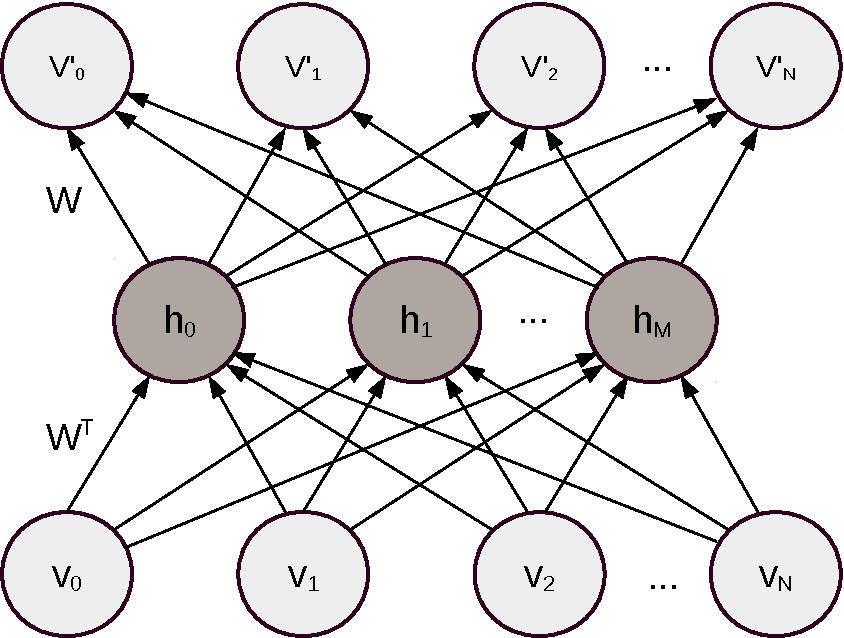
\includegraphics[width=0.5\textwidth]{pics_sdlm/AE.pdf}
	\caption{A typical Autoencoder structure.}
	\label{fig:AE}
\end{figure}

%TODO why tied weights are good
Notice that the connections used in the example are tied weights.

Training an autoencoder is not different from backpropagation (BP) on an Multi-Layer Perceptrons(MLP).
The objective of training is to minimise the prediction error of an MLP, which measured as a loss function.
Accordingly, the loss function of an autoencoder can be described as:
\begin{equation}
L=\sum_{k=1}^{K}\|\mathbf{v}_{k}-\mathbf{v'}_{k}\|=\frac{1}{2}\sum_{k=1}^{K}(\mathbf{v}_{k}-\mathbf{v'}_{k})^{2}
\end{equation}
where k indicates the index of the training data $\mathbf{v}$, and each data vector $\mathbf{v}=\{v_0, v_1,...,v_N\}$ and its reconstruction $\mathbf{v'}=\{v'_0, v'_1,...,v'_N\}$ have N dimensions. 

%TODO rewording
Backpropagation, an abbreviation for "backward propagation of errors", is a common method of training artificial neural networks used in conjunction with an optimization method such as gradient descent.
The method calculates the gradient of a loss function with respect to all the weights in the network.
The gradient is fed to the optimisation method which in turn uses it to update the weights, in an attempt to minimize the loss function:
\begin{equation}
\Delta W \propto -\frac{\partial L}{\partial W}.
\end{equation}

Applying stochastic gradient descent (SGD), the true gradient of the weight matrix, $\Delta W$, is approximated by a gradient at a single example with iterations.
The reconstruction error $E_k$ of an input vector $\mathbf{v}_k$ is as given:
\begin{equation}
%	\begin{align*}
E_k = \frac{1}{2}(\mathbf{v}_k - \mathbf{v'}_k)^2,
%	\end{align*}
\end{equation}
and the gradient of the weight matrix is:
\begin{equation}
\Delta W \propto -\frac{\partial E_k}{\partial W}=-\eta \frac{\partial E_k}{\partial W},
\end{equation}
where $\eta$ is the learning rate.

Since we use tied weights in the network, the weight tuning only needs to apply in the output layer.
\begin{equation}
\begin{aligned}
\Delta w_{ij} = -\eta \frac{\partial E_k}{\partial w_{ij}} &= -\eta \frac{\partial E_k}{\partial v'_j} \frac{\partial v'_j}{\partial net\_v'_j} \frac{\partial net\_v'_j}{\partial w_{ij}}, \textrm{ where} \\
\frac{\partial E_k}{\partial v'_j} &= \frac{\partial \frac{1}{2}(\mathbf{v}_k - \mathbf{v'}_k)^2}{\partial v'_j}= -(v'_j - v_j), \\
%	\frac{\partial v'_j}{\partial net\_v'_j} &= \begin{cases} 1, v'_j>0\\0, v'_j<=0\\ \end{cases}, \textrm{using ReLU,}\\
\frac{\partial v'_j}{\partial net\_v'_j} &= 1, \textrm{using Identify function,}\\
\frac{\partial net\_v'_j}{\partial w_{ij}} &= \frac{\partial h_i w_{ij}}{\partial w_{ij}} = h_i.
\end{aligned}
\end{equation}
Thus, the weight gradient is calculated as:
\begin{equation}
\Delta w_{ij} = \eta h_i(v'_j - v_j)
\end{equation}

Examples of using an autoencoder with 10 input neurons and 10 hidden neurons: reconstruction the input data $\mathbf{v}$ where I) $v_i = 1$, II) $v_i = i/10$.
	\begin{figure}
		\centering
		\begin{subfigure}[t]{0.4\textwidth}
			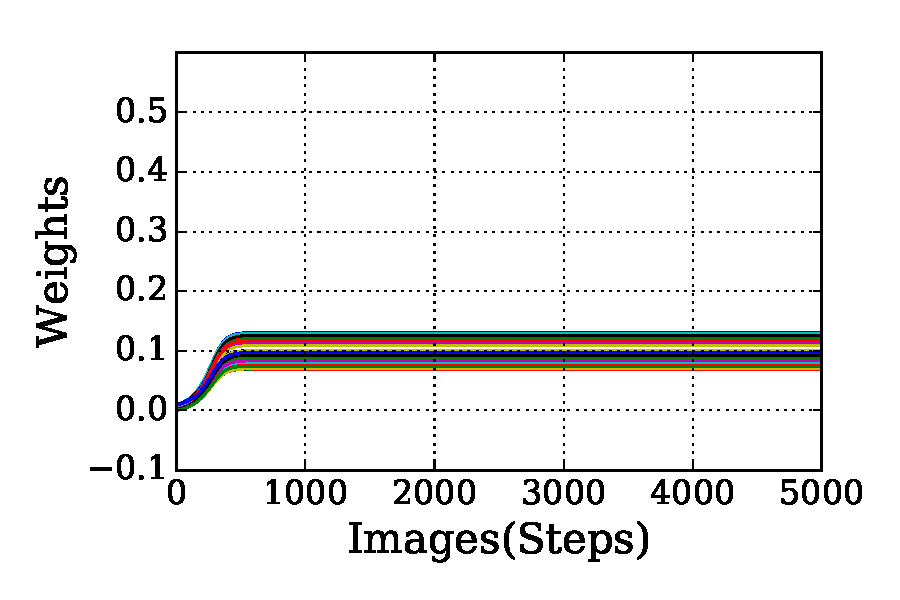
\includegraphics[width=\textwidth]{pics_sdlm/20_exp_AE/exp1_weights_non.pdf}
			\caption{Weights of Exp1}
		\end{subfigure}
		\begin{subfigure}[t]{0.4\textwidth}
			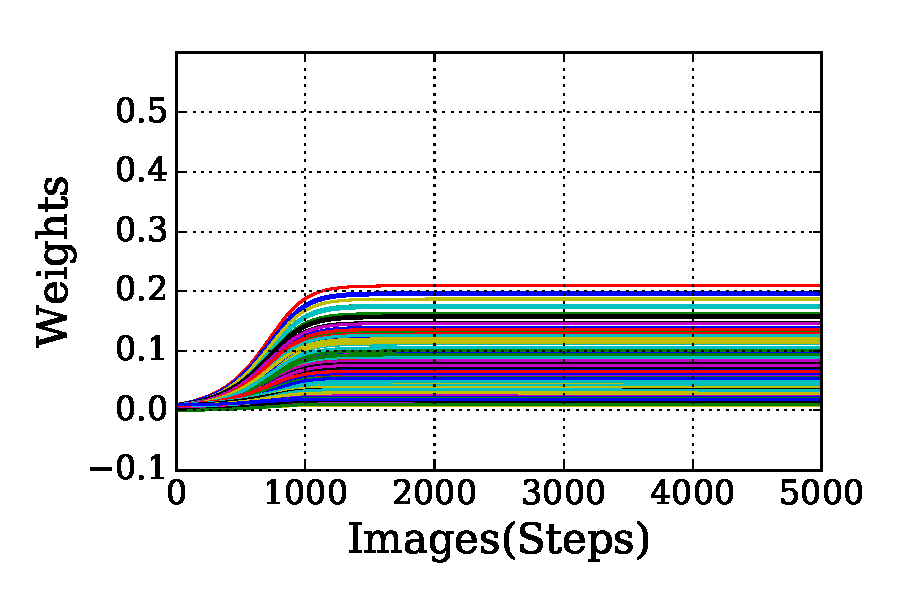
\includegraphics[width=\textwidth]{pics_sdlm/20_exp_AE/exp2_weights_non.pdf}
			\caption{Weights of Exp2}
		\end{subfigure}
		\begin{subfigure}[t]{0.4\textwidth}
			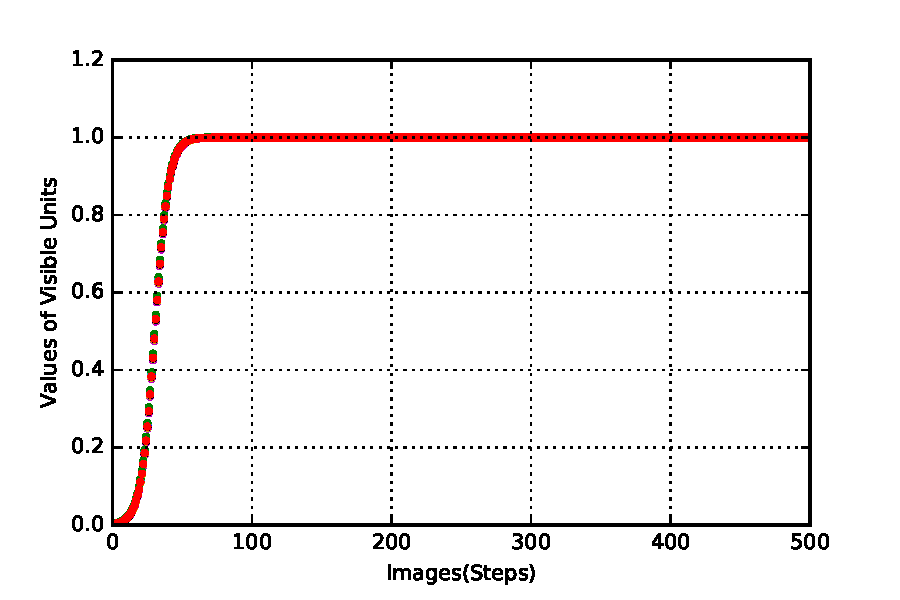
\includegraphics[width=\textwidth]{pics_sdlm/20_exp_AE/exp1_recon_non.pdf}
			\caption{Reconstruction of visible units in Exp1}
		\end{subfigure}
		\begin{subfigure}[t]{0.4\textwidth}
			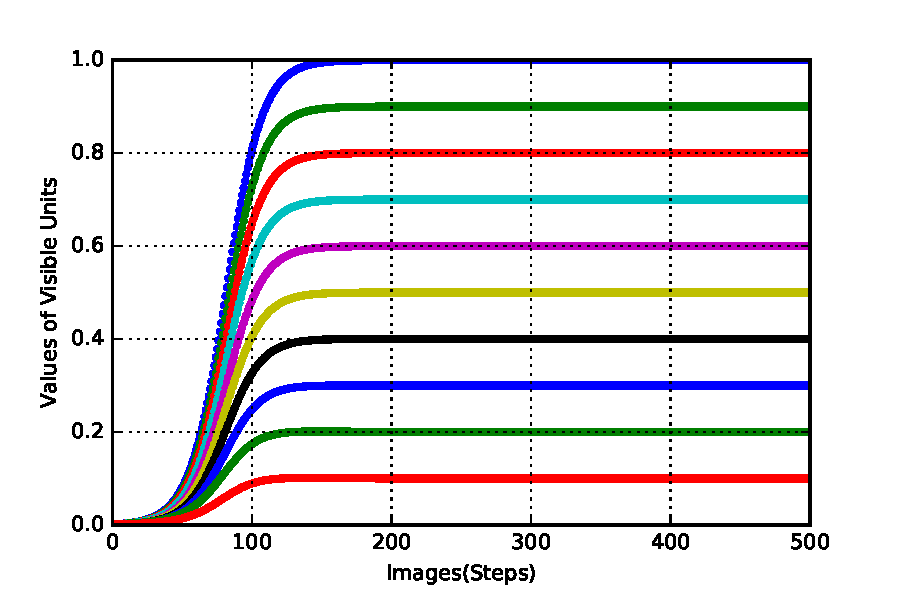
\includegraphics[width=\textwidth]{pics_sdlm/20_exp_AE/exp2_recon_non.pdf}
			\caption{Reconstruction of visible units in Exp2}
		\end{subfigure}\\
		\begin{subfigure}[t]{0.4\textwidth}
			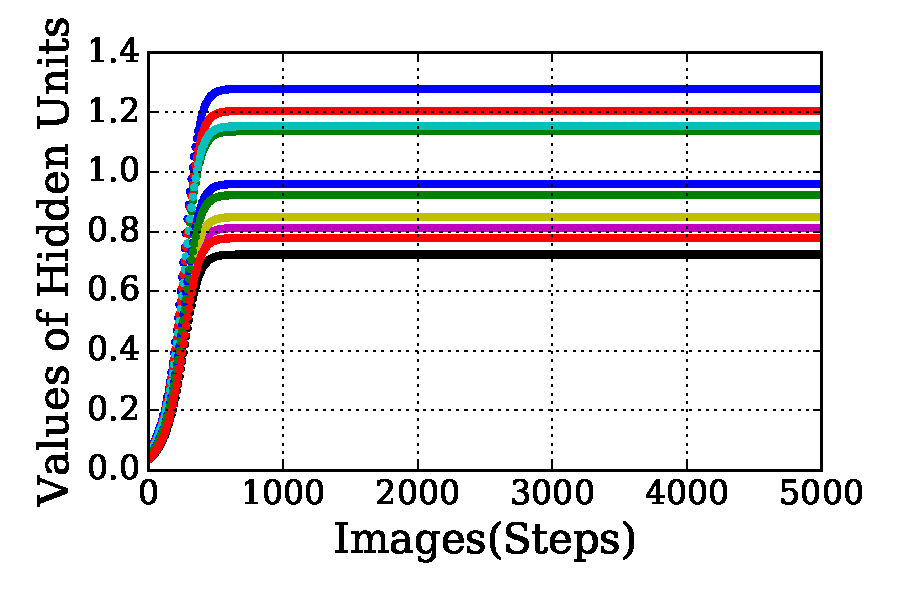
\includegraphics[width=\textwidth]{pics_sdlm/20_exp_AE/exp1_hid_non.pdf}
			\caption{Output of hidden units in Exp1}
		\end{subfigure}
		\begin{subfigure}[t]{0.4\textwidth}
			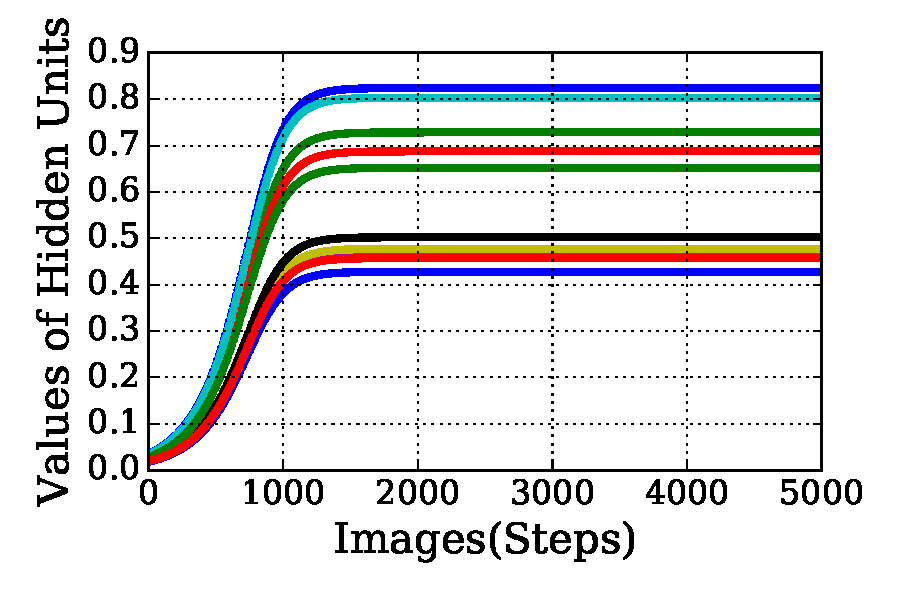
\includegraphics[width=\textwidth]{pics_sdlm/20_exp_AE/exp2_hid_non.pdf}
			\caption{Output of hidden units in Exp2}
		\end{subfigure}\\
		\begin{subfigure}[t]{0.4\textwidth}
			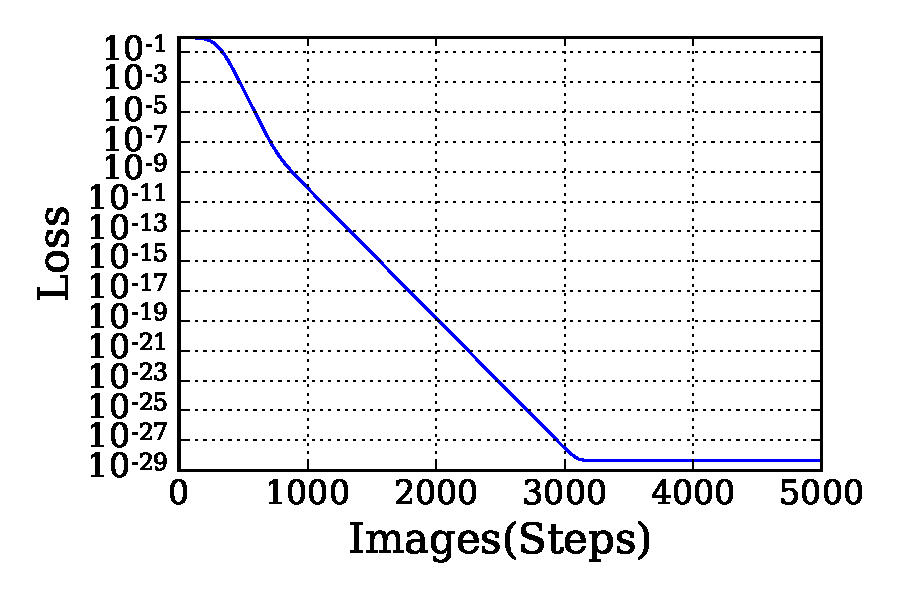
\includegraphics[width=\textwidth]{pics_sdlm/20_exp_AE/exp1_loss.pdf}
			\caption{Output of hidden units in Exp1}
		\end{subfigure}
		\begin{subfigure}[t]{0.4\textwidth}
			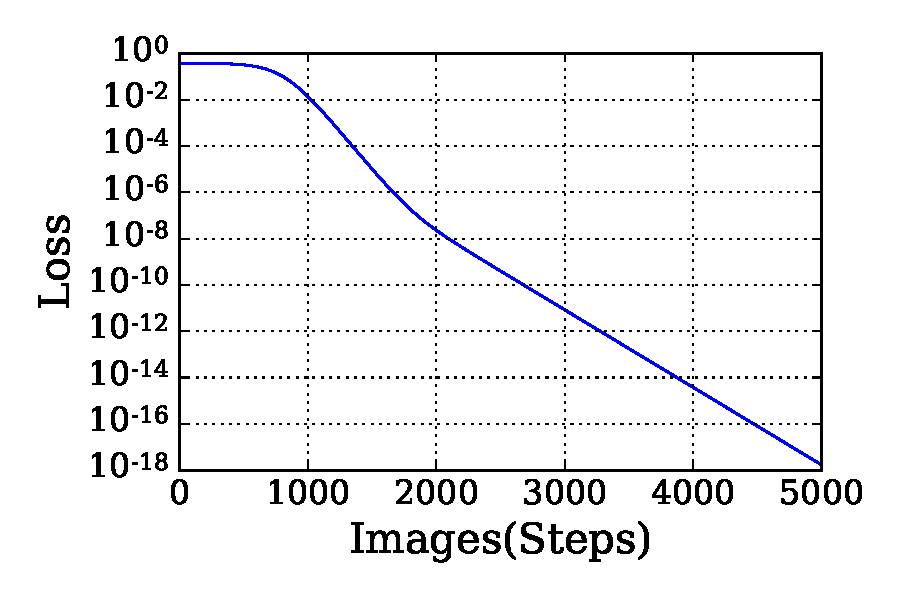
\includegraphics[width=\textwidth]{pics_sdlm/20_exp_AE/exp2_loss.pdf}
			\caption{Output of hidden units in Exp2}
		\end{subfigure}
		\caption{Changes of weights, output of visible and hidden units, and mean squared error (loss) during the AE training of the reconstruction tests. 
			Experiments 1) 10 visible units fully connected to 10 hidden units with input data of all 1s; 2) same network fed with 10 values distribute linearly from 0.1 to 1.}
	\end{figure}



\section{Restricted Boltzmann Machine}
In order to implement training and testing of Spiking Deep~Belief~Networks~(SDBNs) on-line, this section studied:
\begin{itemize}
	\item \textit{Contrastive Divergence.}
	The study starts from understanding the original problem, Products of Experts~(PoE), which was solved by using Contrastive~Divergence~(CD).
	It involves utilising Markov~Chain~Monte~Carlo~(MCMC) sampling to present the distribution of a certain untraceable high-dimensional probability model function, e.g. PoE.
	Among these sampling algorithms, Gibbs method is introduced and used in high dimensional problems.
	Instead of minimising the original objective function of Kullback-Leibler divergence, the contrastive divergence is exploited to solve PoE.
	\item \textit{Restricted Boltzmann Machine (RBM). }
	Then the study continues on applying Gibbs sampling and CD to RBM, which builds the foundation of the light RBM training.
	\item \textit{Deep Belief Network.} 
	The greedy algorithm on training layered RBMs and the fine training on the whole DBN are studied.
\end{itemize}
Next, the study will carry on to on-line learning methods which only applies to spiking neurons for training spiking RBM and DBN.
\subsection{Contrastive Divergence\cite{hinton2002training,woodfordnotes}}
The probability of a vector point $ \mathbf{x} $ is modelled by the function $f(\mathbf{x} \mid \Theta )$ given the model parameters $ \Theta $, and normalised by a partition function $Z( \Theta)$:

\begin{equation}
p(\mathbf{x} \mid \Theta ) = \dfrac{f(\mathbf{x} \mid \Theta )}{Z( \Theta)}
\end{equation}
where the partition function is defined as:
\begin{equation}
\label{equ:z_int}
Z( \Theta) = \int f(\mathbf{x} \mid \Theta )\D\mathbf{x}, \text{when  $ \mathbf{x} $ is continuous, or}
\end{equation}

\begin{equation}
\label{equ:z_dis}
Z( \Theta) = \sum_{\mathbf{x}} f(\mathbf{x} \mid \Theta ), \text{when  $ \mathbf{x} $ is discrete.}
\end{equation}
Given a set of data points $ \mathbf{D}=(\mathbf{d}_1, \mathbf{d}_2, ..., \mathbf{d}_K) $ the purpose of learning is to tune the model parameter $ \Theta $ to fit the data $ \mathbf{D}  $. 
The objective function is the probability product of all the independent data points of the data set, which is also called the likelihood function:
\begin{equation}
L (\Theta \mid \mathbf{D}) = p(\mathbf{D} \mid \Theta ) = \prod_{k=1}^K p(\mathbf{d}_k \mid \Theta ) =  \prod_{k=1}^K\dfrac{f(\mathbf{d}_k \mid \Theta )}{Z( \Theta)}.
\end{equation}
And the target is to maximise the likelihood given the data set $ \mathbf{D}  $, which equals to maximise the log of the probability product (the log-likelihood):
\begin{equation}
\log  L (\Theta \mid \mathbf{D}) = \log p(\mathbf{D} \mid \Theta ) = \sum_{k=1}^K\log f(\mathbf{d}_k \mid \Theta ) - K \log Z( \Theta),
\end{equation}
or the average log-likelihood:
\begin{equation}
\label{equ:like}
\hat{l} (\Theta \mid \mathbf{D}) =\frac{1}{K}\log  L (\Theta \mid \mathbf{D}) 
=\frac{1}{K}\sum_{k=1}^K\log f(\mathbf{d}_k \mid \Theta ) - \log Z( \Theta).
\end{equation}
Imagine three different conditions (probability function) as following.

\textbf{First}, $f(\mathbf{x} \mid \Theta )$ is the probability density function (pdf) of a normal distribution $\mathcal{N}(x \mid \mu, \sigma )$.
Data vector $ \mathbf{x} $ is just a one dimensional data point, $x$.
$ Z( \Theta) $ equals to 1, thus $p(x \mid \Theta ) = \mathcal{N}(x \mid \mu, \sigma )$.
\begin{equation}
\hat{l} (\Theta \mid D) =  
\frac{1}{K} \sum_{k=1}^K \log \left[ \frac{1}{\sigma \sqrt{2\pi}} \exp(-\frac{(d_k-\mu)^{2}}{2\sigma^{2}}) \right]
\label{pdf}
\end{equation}
To maximise Equation~\ref{pdf} is to find the Maximum Likelihood Estimation (MLE) of parameters $ \mu $ and $ \sigma $, by deriving from the partial differential equations when they are equal to 0. 
\begin{equation}
\left\{
\begin{aligned}
&\dfrac{\partial \hat{l} (\Theta \mid D)}{\partial \mu}= \sum_{k=1}^K -\frac{1}{2\sigma^{2}}\dfrac{\partial (\mu-d_k)^{2}}{\partial \mu} = \sum_{k=1}^K -\frac{1}{\sigma^{2}}(\mu-d_k) = 0 \quad\\
&\dfrac{\partial \hat{l} (\Theta \mid D) }{\partial \sigma^{2}}= -\frac{K}{2\sigma^{2}}+\frac{1}{2\sigma^{4}}\sum_{k=1}^K d_k^{2} -\frac{\mu}{\sigma^{4}}\sum_{k=1}^K d_k + \frac{K\mu^{2}}{2\sigma^{4}} = 0 \quad\\
\end{aligned}
\right.
\end{equation}
\begin{equation}
\left\{
\begin{aligned}
&\mu= \frac{1}{K}\sum_{k=1}^K d_k  \quad\\
&\sigma^{2} = \frac{1}{K}\sum_{k=1}^K d_k^{2} - (\frac{1}{K}\sum_{k=1}^K d_k)^{2}
\end{aligned}
\right.
\end{equation}
$\hat{l} (\Theta \mid D)$ here is the function of two dimensional parameters $\mu$ and $\theta$, and searching the highest point in the parameter space ``is equivalent to being in the field on a clear, sunny day,''~\cite{woodfordnotes} seeing the point straight away.

\textbf{Second}, the probability model function changes to be the sum of N normal distributions: 
\begin{equation}
f(x \mid \Theta ) = \sum_{i=1}^N\mathcal{N}(x \mid \mu_i, \sigma_i ).
\end{equation}
Derived from Equation~(\ref{equ:like}), the objective function is:
\begin{equation}
\hat{l} (\Theta \mid D) = \frac{1}{K}\sum_{k=1}^K \log \sum_{i=1}^N \mathcal{N}(d_k \mid \mu_i, \sigma_i ) - \log N,
\end{equation}
where $\log Z( \Theta)$ still equals a constant, but the partial differential equation of any parameter depends on other model parameters.
It is very hard to solve equation set of log of sum, thus iteration methods are introduced, e.g., gradient descent method. %and expectation maximization (EM) algorithm
Searching for a local maximum of the likelihood function in the parameter space starts with an initial point, either random or well selected.
For each iteration, the partial derivatives for every dimension of the parameter point are calculated as the gradient.
The gradient determines the decent direction of the space search, the next parameter point is one step $ \eta $  towards the direction or is the highest point found by line search.

The gradient descent method is equivalent to ``being in the field at night with a torch.''~\cite{woodfordnotes}.
And then the descent direction is estimated and chosen by using the torch to see the relative heights of the field a short distance in each direction.
Because partial differential equation of any parameter depends on other model parameters, we can only see the gradient for a small area.
The search will follow the direction by walking one step or a certain distance (e.g. line search lowest point), and then start a new iteration.


\subsubsection{PoE Problem}
\textbf{Finally}, the probability model function becomes the product of N normal distributions: 
\begin{equation}
f(x \mid \Theta ) = \prod_{i=1}^N\mathcal{N}(x \mid \mu_i, \sigma_i ),
\end{equation}
where the partition (normalisation) function $Z( \Theta)$ is no longer a constant, but varies accordance to all the parameters.
Essentially, the integration of the probability model, see Equation~(\ref{equ:z_int}) and~(\ref{equ:z_dis}), is usually algebraically intractable.
We have to use numerical integration method to evaluate the Equation~(\ref{equ:like}), whose partial derivative is (we are using vectors to generalise the problem):
\begin{equation}
\label{equ:part}
\begin{aligned}
\dfrac{\partial \hat{l} (\Theta \mid \mathbf{D})}{\partial \theta} 
& = \frac{1}{K} \dfrac{\partial \sum_{k=1}^K\log f(\mathbf{d}_k \mid \Theta )}{\partial \theta} - \dfrac{\partial \log Z( \Theta)}{\partial \theta}\\
& =  \frac{1}{K}\sum_{k=1}^K \dfrac{\partial \log f(\mathbf{d}_k \mid \Theta)}{\partial \theta} - \int p(\mathbf{x} \mid \Theta) \dfrac{\partial \log f(\mathbf{x} \mid \Theta)}{\partial \theta} \D \mathbf{x}\\
& = \left \langle \dfrac{\partial \log f(\mathbf{d} \mid \Theta)}{\partial \theta}\right \rangle_{\mathbf{D}} -\left \langle \dfrac{\partial \log f(\mathbf{c} \mid \Theta)}{\partial \theta}\right \rangle_{\mathbf{C} \sim p(\mathbf{x} \mid \Theta)}  \\
&=\left \langle \dfrac{\partial \log f(\mathbf{x} \mid \Theta)}{\partial \theta}\right \rangle_{\mathbf{X}_{data}} - \left \langle \dfrac{\partial \log f(\mathbf{x} \mid \Theta)}{\partial \theta}\right \rangle_{\mathbf{X}_{model}},
\end{aligned}
\end{equation}
where  $ <\cdot>_x $ denotes the mean expectation of $ \cdot $ given distribution of $x$.
The first term of the right-hand side is easy to get with the given data set $ \mathbf{D} $, and the second term can be approximated by generating data samples $ \mathbf{C} $ according to $ p(\mathbf{x} \mid \Theta) $.
These generative samples is called ``fantasy data'' and can be generated using Monte Carlo Markov Chain (MCMC) sampling, see section~\ref{sec:mcmc}.
The detailed derivation process can be found in Appendix~\ref{app:part}.
Although in this example the integration of product of normal distribution is still tractable, it is also helpful to use numerical integration.

Go back to the metaphor of the parameter field, solving PoE problem is like searching the highest point in a completely dark night without a torch.
The computation of Equation~(\ref{equ:part}) is to ``feel the gradient of the field under our feet''.~\cite{woodfordnotes}.
%The motivation underlining Contrastive Divergence algorithm is to boost the training speed of a Markov Chain in order to represent the distribution of a PoE (Product of Expert) model.
%Thus the sampling can be followed using this trained Markov Chain model. 
\subsubsection{MCMC Sampling}
\label{sec:mcmc}
In order to solve the integration of algebraically intractable equations we can use numerical integration to approximate.
One of the popular method is Monte Carlo integration:
\begin{equation}
\int_{a}^{b} f(x) \D x = \int_{a}^{b}\frac{f(x)}{q(x)}q(x)\D x = \dfrac{1}{N}\sum_{i=1}^{N}\frac{f(x_i)}{q(x_i)}.
\end{equation}
The integration of $ f(x) $ transforms to the integration of a new function $ F(x) = f(x)/q(x)  $ times its probability function $ q(x) $.
It could be approximated by sampling N data points $ x_i $ according to the probability distribution $ q(x) $, and calculate the average of $ F(x_i) $ as $ <F(x)>_{q(x)}$.
So the main question following is how to sample from a probability distribution.

MCMC algorithm was proposed by Metropolis in 1953 and it became a wide-used sampling method.
The stationary distribution $ \pi $ exists when every two nodes in a Markov Chain are connected regardless of the initial state distribution $ \pi_0 $:
\begin{equation}
\begin{aligned}
&\pi(j) = \sum_{i=1}^{\infty}\pi(i)P_{ij} \\
&\pi P = \pi,
\end{aligned}
\end{equation}
where $ P $ is the transition probability matrix, and $ \pi $ is in the state space of a MC and the sum, $ \sum_{i=1}^{\infty}\pi(i) $,of a state distribution is 1.
Thus based on the useful theorem of MC, sampled sequence $ \{x_0, x_1, ..., x_n, ... \}$ from a MC complies with its stationary distribution $ \pi(x) $.
Metropolis stated that if a MC has a stationary distribution, $ q(x) $, which is exactly needed to sample from, then we can easily obtain a sample sequence along the MC according to the transformation probability matrix $ P $.
Here so far we are describing the MC with discrete states, however the it also applies to continuous $ \pi $ and $ P $.
The problem here is to build $ P $ to make the stationary distribution equal to the required probability, $ \pi(x) = q(x) $.

So the other useful theorem (detailed balance) lies here, if an aperiodic MC is reversible: $\pi (i) P_{ij} = \pi (j) P_{ji},$ then $ \pi $ is the stationary distribution.
It is a stronger condition than the previous theorem, so most of the MCs are not generally eligible:
\begin{equation}
\pi (i) P_{ij} \neq \pi (j) P_{ji}.
\end{equation}
Thus we can introduce another parameter matrix, $ \alpha $ to make a general MC reversible:
\begin{equation}
\pi (i) P_{ij} \alpha_{ij} = \pi (j) P_{ji} \alpha_{ji}	,
\end{equation}
where $ \alpha_{ij} = \pi(j) P_{ji} $ and $ \alpha_{ji} = \pi(i) P_{ij}$.
The altered transformation probability matrix is $ P'_{ij} =  P_{ij} \alpha_{ij}$ and $ P'_{ji} =  P_{ji} \alpha_{ji}$, and the MC complies the detailed balance condition: $\pi (i) P'_{ij} = \pi (j) P'_{ji}$.
The matrix parameter $ \alpha $ is called as ``acceptance rate'', and its physic meaning is as follows: when state $ i $ transforms to state $ j $ with a probability of $ P_{ij} $, the transformation is accepted by the rate of $ \alpha_{ij} $.
Since the accept rate may be too low for the sampling to move along the MC, we can normalise the $ \alpha $ pair to 1:
\begin{equation}
\alpha^{'}(i,j) = min \left\{\frac{\pi(j)P_{ji}}{\pi(i)P_{ij}},1\right\}.
\end{equation}
The algorithm is called Metropolis-Hastings and described in following:
\begin{algorithm}[h]
	\caption{Metropolis-Hastings Sampling}
	\label{alg:mcmc}
	\begin{algorithmic}
		
		%	    \Procedure{Correction}{coeffs $C$, correlations $Q$}
		\State Initialisation $x_0 = s_{random}$, \Comment{$ x $:sampling sequence and $s$:state in MC}
		\For{$t=1, 2, ..., N$}
		\State $y \sim p_(x \mid x_{t-1})$ 
		\Comment{Random drawing the next state by the transformation probability matrix $P$}
		\State $ u \sim Uniform[0,1] $ 
		\Comment{Random drawing from a uniform distribution}
		\If {$ u < \alpha^{'}(x_{t-1},y) = min \left\{\frac{q(y)p_(x_{t-1} \mid y)}{q(x_{t-1})p_(y \mid x_{t-1})},1\right\} $}
		\State {$x_t = y$} \Comment{Accept the transformation when the random number is less than $\alpha$}
		\Else \State {$x_t = x_{t-1}$}  \Comment{Transformation is refused elsewise}
		\EndIf
		\EndFor
	\end{algorithmic}
\end{algorithm}

The probability model function as the product of N normal distributions can be approximated by using this Metropolis-Hastings sampling.
\subsubsection{Gibbs Sampling}
\label{sec:Gibbs}
For high dimensional data sampling, it is possible to make the accept rate to 1 which increases the convergence speed dramatically.
According to conditional probability:
\begin{equation}
P(A \mid B) = \frac{P(A \cap B)}{P(B)}.
\end{equation}
For a $ n $ dimensional data $ (\mathbf{x}, y) $ where $ \mathbf{x}=(x_1,x_2,...,x_{n-1}) $, the joint probability of $p(\mathbf{x},y)$ is:
\begin{equation}
p(\mathbf{x},y) = p(y \mid \mathbf{x})p(\mathbf{x}).
\end{equation}
Thus, during sampling if we restrict the direction of transformation to one single axis(dimension), $ y $, from point $ A(\mathbf{x}_1, y_1) $ to point $ B(\mathbf{x}_1, y_2)$:
\begin{equation}
p(\mathbf{x}_1, y_1)p(y_2 \mid \mathbf{x}_1) = p(\mathbf{x}_1, y_2)p(y_1 \mid \mathbf{x}_1) = p(\mathbf{x}_1)p(y_1 \mid \mathbf{x}_1)p(y_2 \mid \mathbf{x}_1),
\end{equation}
then, the MC obeys the condition of detailed balance.
So the stationary distribution $ \pi(x_1,x_2,...,x_n) $ equals to the joint probability $ p(x_1,x_2,...,x_n) $ and the transformation probability matrix P is consisted of the conditional probability of each dimension $ k $ $,  p(x_k \mid x_1,...,x_{k-1},x_{k+1},...,x_n) $.
Therefore, given the conditional distribution of each variable for a multivariate distribution Gibbs sampling is able to approximate the joint distribution with long enough sample sequence.
Gibbs sampling is described as follows:
\begin{algorithm}[h]
	\caption{Gibbs Sampling}
	\label{alg:gibbs}
	\begin{algorithmic}
		
		%	    \Procedure{Correction}{coeffs $C$, correlations $Q$}
		\State Initialisation $\mathbf{x}_0 = [x_0(1),x_0(2),...,x_0(M)]$,  \Comment{Random initialise $\mathbf{x}_0$}
		\For{$t=1, 2, ..., N$}
		\For{$k=1, 2, ..., M$}
		\State $ x_t(k) = p(x(k) \mid x_{t-1}(1),x_{t-1}(2),...,x_{t-1}(k-1),x_{t-1}(k+1),...,x_{t-1}(M))$\\
		\Comment{Sampling by the conditional distribution}
		\EndFor
		\EndFor
	\end{algorithmic}
\end{algorithm}

\subsubsection{CD Instead of KL(Kullback-Leibler)}
\label{sec:CD}
Kullback-Leibler divergence is the measure of how different two probability distributions are:
\begin{equation}
\begin{aligned}
KL(P \mid \mid Q)
&= \int P(\mathbf{x}) \log \frac{P(\mathbf{x})}{Q(\mathbf{x})} \D \mathbf{x}\\
%= \sum_{\mathbf{x}} P(\mathbf{x}) \log \frac{P(\mathbf{x})}{Q(\mathbf{x})} \\
&= \int P(\mathbf{x}) \log P(\mathbf{x}) \D \mathbf{x} - \int P(\mathbf{x}) \log Q(\mathbf{x}) \D \mathbf{x}\\
%=  \sum_{\mathbf{x}} P(\mathbf{x}) \log P(\mathbf{x}) - \sum_{\mathbf{x}} P(\mathbf{x}) \log Q(\mathbf{x})\\
&= \left \langle \log P(\mathbf{x}) \right \rangle_{\mathbf{X} \sim P(\mathbf{x})} - \left \langle \log Q(\mathbf{x}) \right \rangle_{\mathbf{X} \sim P(\mathbf{x})} ,
\end{aligned}
\end{equation}
and the second term of the right hand side is the average log-likelihood function (see Equation~\ref{equ:like}) if $P(\mathbf{x})$ is the training data distribution and $Q(\mathbf{x})$ is the model distribution:
\begin{equation}
\begin{aligned}
& KL \left( p(\mathbf{x} \mid \mathbf{D}) \mid \mid p(\mathbf{x} \mid \Theta) \right)
=   \left \langle \log p(\mathbf{d} \mid \mathbf{D}) \right \rangle_{\mathbf{D}} - \left \langle \log p(\mathbf{d} \mid \Theta) \right \rangle_{\mathbf{D}}, \textit{where} \\
& \hat{l} (\Theta \mid \mathbf{D}) =\frac{1}{K}\log  L (\Theta \mid \mathbf{D}) 
=  \frac{1}{K}\log p(\mathbf{D} \mid \Theta ) 
= \frac{1}{K} \sum_{k=1}^{\mathbf{K}} \log f(\mathbf{d}_k \mid \Theta )
= \left \langle \log p(\mathbf{d} \mid \Theta) \right \rangle_{\mathbf{D}}.
\end{aligned}
\end{equation}
We use $ \mathbf{D} $ instead of $ \mathbf{X} \sim p(\mathbf{x} \mid \mathbf{D}) $, for $ p(\mathbf{x} \mid \mathbf{D}) $ is the distribution of data set $ \mathbf{D} $.
If we need to generate a sample sequence according to the distribution $ p(\mathbf{x} \mid \mathbf{D}) $, $ \mathbf{D} $ itself is the most approximated.
Since $\left \langle \log p(\mathbf{d} \mid \mathbf{D}) \right \rangle_{\mathbf{D}}$ is independent with model parameters, the negative partial derivative is the same with Equation~(\ref{equ:part}):
\begin{equation}
\label{equ:kl}
-\dfrac{\partial KL \left( p(\mathbf{x} \mid \mathbf{D}) \mid \mid p(\mathbf{x} \mid \Theta) \right)}{\partial \theta}
= \dfrac{\partial \hat{l} (\Theta \mid \mathbf{D})}{\partial \theta} \\
= \left \langle \dfrac{\partial \log f(\mathbf{d} \mid \Theta)}{\partial \theta}\right \rangle_{\mathbf{D}} - \left \langle \dfrac{\partial \log f(\mathbf{c} \mid \Theta)}{\partial \theta}\right \rangle_{\mathbf{C} \sim p(\mathbf{x} \mid \Theta)} .
\end{equation}
Therefore, for each iteration searching in the parameter space we use $ k $ number of training data $ \mathbf{D}=(\mathbf{d}_1, \mathbf{d}_2, ..., \mathbf{d}_k) $ and fantasy data $ \mathbf{C}=(\mathbf{c}_1, \mathbf{c}_2, ..., \mathbf{c}_k) $.
If $ k $ is big enough, sampling sequences $ \mathbf{D} $ and $ \mathbf{C} $ are able to approximate the data and the model distribution thus to get derivatives of the KL function.
However, if we just take a small number of data, even $ k = 1 $ per iteration~\cite{hinton2002training}, the KL divergence can be seen as a ``k-step contrastive convergence ($ CD_{k}) $'':
\begin{equation}
\label{equ:cdk}
\dfrac{\partial CD_{k}}{\partial \theta} 
= - \left \langle \dfrac{\partial \log f(\mathbf{d} \mid \Theta)}{\partial \theta}\right \rangle_{(\mathbf{d}_1, \mathbf{d}_2, ..., \mathbf{d}_k) } + \left \langle \dfrac{\partial \log f(\mathbf{c} \mid \Theta)}{\partial \theta}\right \rangle_{(\mathbf{c}_1, \mathbf{c}_2, ..., \mathbf{c}_k) \sim p(\mathbf{x} \mid \Theta)}.
\end{equation}
Since the searching step $ \eta $ is very small, the derivatives of points in a small area can be seen as the same.
%	The step made for a single $ CD_{k} $ can be approximated by summation of $ k $ steps of $ CD_{1} $ as long as the searching does not go far.
%	Otherwise the searching path may follow some direction for accumulated steps away from the original area, thus significantly reduces the training time.

\subsubsection{Discussion}
Although there is practical explanation on using $CD_1$ for parameter space searching, arguments exist over whether the search converge to the same maxima/minima as $CD_\infty$~\cite{wu2015bias}.
Moreover, is the parameter searching still following the original objective function?	
As an initial exploration over the problem we tested some experiments on Section~\ref{sec:cd1}. 
%	Thus,
%	\begin{equation}
%		\dfrac{\partial [KL(p^0 \mid \mid p^{\infty}) - KL(p^1 \mid \mid p^{\infty})]}{\partial \theta}
%		= \left \langle \dfrac{\partial \log f(\mathbf{x} \mid \Theta)}{\partial \theta}\right \rangle_{\mathbf{p}^1} - \left \langle \dfrac{\partial \log f(\mathbf{x} \mid \Theta)}{\partial \theta}\right \rangle_{\mathbf{p}^0},
%	\end{equation}
%	where the second term in equation~(\ref{equ:kl}) cancels out.
%	So Hinton proposed \textcolor{red}{the new contrastive divergence CD to make Gibbs sampling with only 1 step}.
%	Contrastive divergence is defined as:
%	\begin{equation}
%		CD_n = KL(p^0 \mid \mid p^{\infty}) - KL(p^n \mid \mid p^{\infty})
%	\end{equation}
\subsection{RBM\cite{zhang2013rbm}}
RBM is a restricted version of Boltzman machine, where there are only connections between layers of units but not between units within a layer, see Figure~\ref{fig:RBM}.
$ v $ is the layer of visible units representing the observable data $ \mathbf{v} $, while $ h $ are the hidden units which can be seen as feature extractors.
The connections between the hidden layer and the visible layers are bidirectional weights, $ \mathbf{W} $.
Note that, both visible and hidden units have their bias individually, $ \mathbf{a} $ and $ \mathbf{b} $.
Thus the RBM consists of the data $ \mathbf{D} = \mathbf{V} = (\mathbf{v}_1, \mathbf{v}_2, ..., \mathbf{v}_K ) $, the model parameters $ \Theta = (\mathbf{a}, \mathbf{b}, \mathbf{W}) $ and the hidden units $ \mathbf{h} \sim p(\mathbf{h} \mid \mathbf{v}, \Theta) $.
\begin{figure}[hbt]
	\centering
	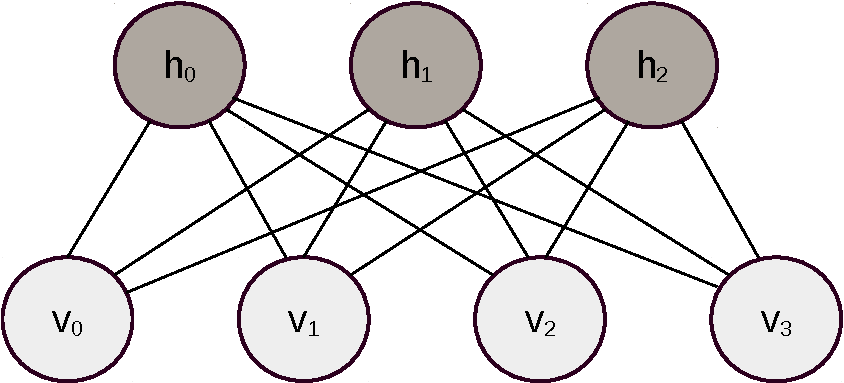
\includegraphics[width=0.6\textwidth]{pics_sdbn/RBM.pdf}
	\caption{A typical RBM structure.}
	\label{fig:RBM}
\end{figure}

The Energy function~\cite{hopfield1982neural} of a RBM is defined as follows, which has $ n $ vision units and $ m $ hidden ones:
\begin{equation}
E(\mathbf{v}, \mathbf{h} \mid \Theta)= -\sum_{i=1}^n a_i v_i - \sum_{j=1}^m b_j h_j - \sum_{i=1}^n \sum_{j=m}^n v_i W_{ij} h_j.
\end{equation}
And the model function and its probability functions are as follows:
\begin{equation}
\begin{aligned}
& f(\mathbf{v}, \mathbf{h} \mid \Theta) =e^{-E(\mathbf{v}, \mathbf{h} \mid \Theta)} \\
& p(\mathbf{v}, \mathbf{h} \mid \Theta) =\frac{e^{-E(\mathbf{v}, \mathbf{h} \mid \Theta)}}{Z(\Theta)}\\
& Z(\Theta) = \sum_{\mathbf{v}} \sum_{\mathbf{h}} e^{-E(\mathbf{v}, \mathbf{h} \mid \Theta)}.
\end{aligned}
\end{equation}
Note that, the model function $ f(\mathbf{v}, \mathbf{h} \mid \Theta) $ is nicely defined as a PoE problem, and each hidden unit represent an expert.
However, we are more interested in the marginal probability function: $ p(\mathbf{v} \mid \Theta) $:
\begin{equation}
p(\mathbf{v} \mid \Theta) =\frac{\sum_{ \mathbf{h}} e^{-E(\mathbf{v}, \mathbf{h} \mid \Theta)}}{Z(\Theta)}.
\end{equation}		
\subsubsection{Objective Function}
Although $ p(\mathbf{v} \mid \Theta) $ is not a PoE problem, the partial derivation of the average log-likelihood function still applies to Equation~(\ref{equ:part}) and the intractable integration is the same problem here:
\begin{equation}
\label{equ:RBM}
\begin{aligned}
\dfrac{\partial \hat{l} (\Theta \mid \mathbf{D})}{\partial \theta} 
& = \left \langle \dfrac{\partial -E(\mathbf{v}, \mathbf{h} \mid \Theta)}{\partial \theta} \right \rangle_{\mathbf{h} \sim p( \mathbf{h} \mid \mathbf{v}, \Theta), \mathbf{V}} 
- \left \langle \dfrac{\partial -E(\mathbf{v}, \mathbf{h} \mid \Theta)}{\partial \theta} \right \rangle_{\mathbf{v}, \mathbf{h} \sim p( \mathbf{v}, \mathbf{h} \mid  \Theta)},  \\
\end{aligned}
\end{equation}
The detailed derivation process, please see Appendix~\ref{app:RBM}.
Regarding the specific RBM parameters,  $ \Theta = (\mathbf{a}, \mathbf{b}, \mathbf{W}) $, the derivatives are:
\begin{equation}
\label{equ:RBM_2}
\begin{aligned}
\dfrac{\partial \hat{l} (\Theta \mid \mathbf{D})}{\partial W_{ij}} 
& = \left \langle v_i h_j \right \rangle_{\mathbf{h} \sim p( \mathbf{h} \mid \mathbf{v}, \Theta), \mathbf{V}} 
- \left \langle  v_i h_j \right \rangle_{\mathbf{v}, \mathbf{h} \sim p( \mathbf{v}, \mathbf{h} \mid  \Theta)},  \\
\dfrac{\partial \hat{l} (\Theta \mid \mathbf{D})}{\partial a_{i}} 
& = \left \langle v_i \right \rangle_{\mathbf{h} \sim p( \mathbf{h} \mid \mathbf{v}, \Theta), \mathbf{V}} 
- \left \langle  v_i \right \rangle_{\mathbf{v}, \mathbf{h} \sim p( \mathbf{v}, \mathbf{h} \mid  \Theta)},  \\
\dfrac{\partial \hat{l} (\Theta \mid \mathbf{D})}{\partial b_{j}} 
& = \left \langle h_j \right \rangle_{\mathbf{h} \sim p( \mathbf{h} \mid \mathbf{v}, \Theta), \mathbf{V}} 
- \left \langle  h_j \right \rangle_{\mathbf{v}, \mathbf{h} \sim p( \mathbf{v}, \mathbf{h} \mid  \Theta)},  \\
\end{aligned}
\end{equation}	 
\subsubsection{CD with 1-step Reconstruction}
\label{sec:cd}
Both terms of the derivatives of the average log-likelihood function (Equation~(\ref{equ:RBM})) are intractable, so generative models for sampling is needed.
As stated in Section~\ref{sec:CD}, for each iteration only one sample is generated.

Regarding to the first term, given a training data $ \mathbf{v}_0 $ we first generate a hidden vector according to the conditional distribution $ \mathbf{h}_0 \sim p( \mathbf{h} \mid \mathbf{v}_0, \Theta) $.
Welling et al. have proposed~\cite{welling2004exponential} that both the hidden and visible units can be any exponential unit, such as softmax, Gaussian and Poissonian.
Here we take a Bernoulli-Bernoulli RBM as an example, where each node is a sigmoidal unit.
The conditional probability function is as follows:
\begin{equation}
p(h_i = 1 \mid \mathbf{v}) = \sigma(\sum_{j=1}^{m} W_{ij} \cdot \mathbf{v} + b_j).
\end{equation}

\begin{figure}[hbt]
	\centering
	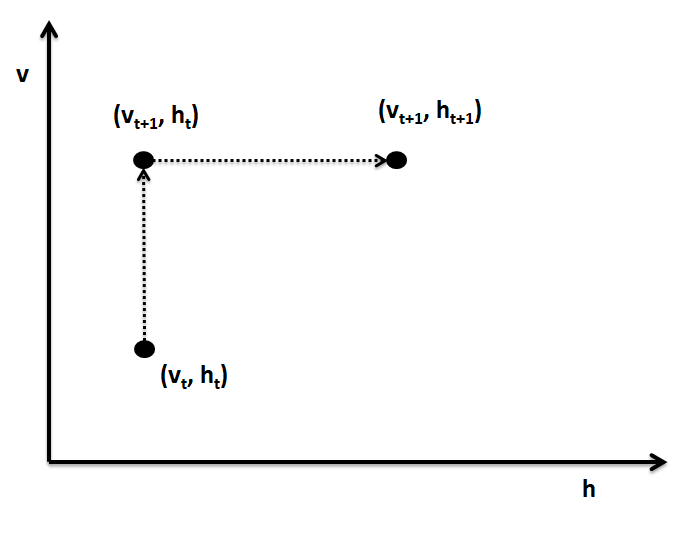
\includegraphics[width=0.6\textwidth]{pics_sdbn/gibbs.png}
	\caption{Gibbs sampling on RBM.}
	\label{fig:gibbs}
\end{figure}
The second term is perfect fit for Gibbs sampling, since we can $ p(\mathbf{v}, \mathbf{h} \mid \Theta) $ as a 2D vector and generating the samples by jumping in a Markov Chain with the transformation probability matrix $ p(\mathbf{v} \mid \mathbf{h}, \Theta) $ and $ p(\mathbf{h} \mid \mathbf{v}, \Theta) $, see Figure~\ref{fig:gibbs} and Section~\ref{sec:Gibbs}.
So, with the given data $ \mathbf{v}_0 $ and the sampling data $ \mathbf{h}_0 $, we have the initial data point in this Markov Chain,  ($ \mathbf{v}_0, \mathbf{h}_0$).
The transformation starts from the axis of $ \mathbf{v} $, then we get $ \mathbf{v}_1 \sim p( \mathbf{v} \mid \mathbf{h}_0, \Theta) $.
It follows the next axis $ \mathbf{h} $, similarly we get $ \mathbf{h}_1 \sim p( \mathbf{h} \mid \mathbf{v}_1, \Theta) $.
So far we obtain the first sample along the Markov Chain, ($ \mathbf{v}_1, \mathbf{h}_1$) thus to solve the objective function with one iteration.
The algorithm is described below:   
\begin{algorithm}[h]
	\caption{Learning on RBM Parameters with $ CD_1 $}
	\label{alg:learn}
	\begin{algorithmic}
		%			\State Initialisation $\mathbf{x}_0 = [x_0(1),x_0(2),...,x_0(M)]$,  \Comment{Random initialise $\mathbf{x}_0$}
		\For{$t=1, 2, ..., K$} \Comment{K number of training data $ \mathbf{V} $, 1 data each iteration}
		%			\For{$k=1, 2, ..., M$}
		\State $ \mathbf{h}_t \sim p( \mathbf{h} \mid \mathbf{v}_t, \Theta) $
		\Comment{Generate $ \mathbf{h}_t $ given $ \mathbf{v}_t $ }
		\State $ \mathbf{v}_{t+1} \sim p( \mathbf{v} \mid \mathbf{h}_{t}, \Theta) $
		\Comment{Generate $ \mathbf{v}_{t+1} $ on v axis using Gibbs sampling }
		\State $ \mathbf{h}_{t+1} \sim p( \mathbf{h} \mid \mathbf{v}_{t+1}, \Theta) $
		\Comment{Generate $ \mathbf{h}_{t+1} $ on h axis using Gibbs sampling }
		\State $ \dfrac{\partial \hat{l} (\Theta \mid \mathbf{D})}{\partial W_{ij}} = v_{t,i} h_{t,j} - v_{t+1,i} h_{t+1,j}$
		\State $ \dfrac{\partial \hat{l} (\Theta \mid \mathbf{D})}{\partial a_{i}} = v_{t,i} - v_{t+1,i} $
		\State $  \dfrac{\partial \hat{l} (\Theta \mid \mathbf{D})}{\partial b_{j}} = h_{t,j} - h_{t+1,j}$
		\State $ \Delta W_{ij} = \eta ( v_{t,i} h_{t,j} - v_{t+1,i} h_{t+1,j}) $
		\Comment{Update $ W_{ij} $}
		\State $ \Delta a_{i} = \eta ( v_{t,i} - v_{t+1,i}) $
		\Comment{Update $ a_{i} $}
		\State $ \Delta b_{j} = \eta ( h_{t,j} - h_{t+1,j}) $
		\Comment{Update $ b_{j} $}
		%			\EndFor
		\EndFor
	\end{algorithmic}
\end{algorithm}
	

\subsection{noisy RBM}
Instead of using binary units in RBM, we employ noisy ReLU units constructing noisy RBM which is closer to biology and performances better in classification tasks\cite{nair2010rectified}.

Examples of using an autoencoder with 10 input neurons and 10 hidden neurons: reconstruction the input data $\mathbf{v}$ where I) $v_i = 1$, II) $v_i = i/10$.
\begin{figure}
	\centering
	\begin{subfigure}[t]{0.4\textwidth}
		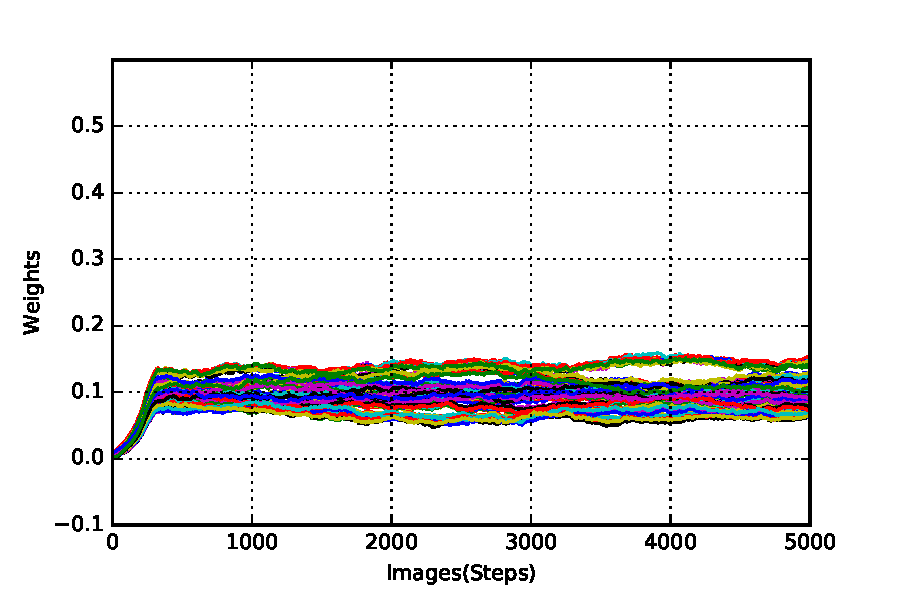
\includegraphics[width=\textwidth]{pics_sdlm/30_exp_RBM/exp1_weights_non.pdf}
		\caption{Weights of Exp1}
	\end{subfigure}
	\begin{subfigure}[t]{0.4\textwidth}
		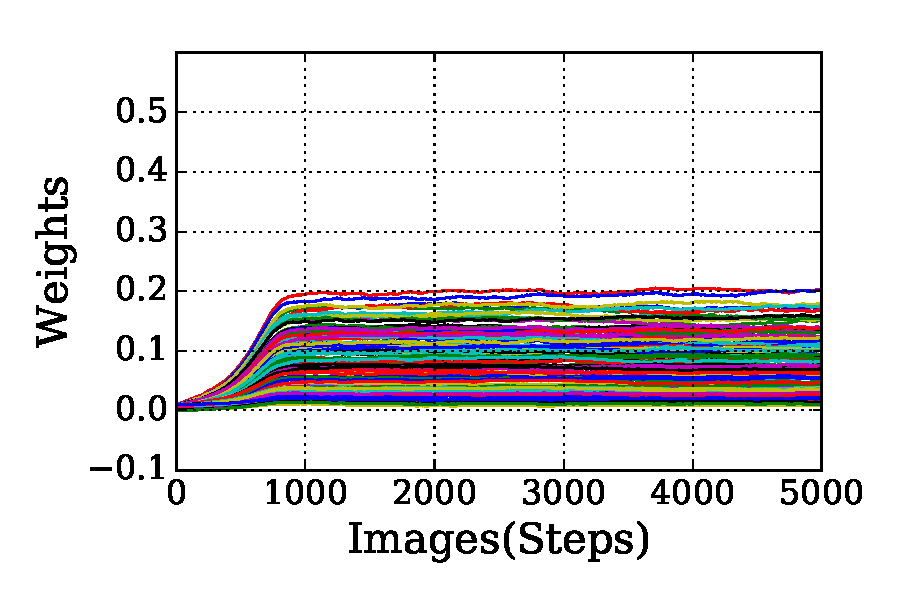
\includegraphics[width=\textwidth]{pics_sdlm/30_exp_RBM/exp2_weights_non.pdf}
		\caption{Weights of Exp2}
	\end{subfigure}
	\begin{subfigure}[t]{0.4\textwidth}
		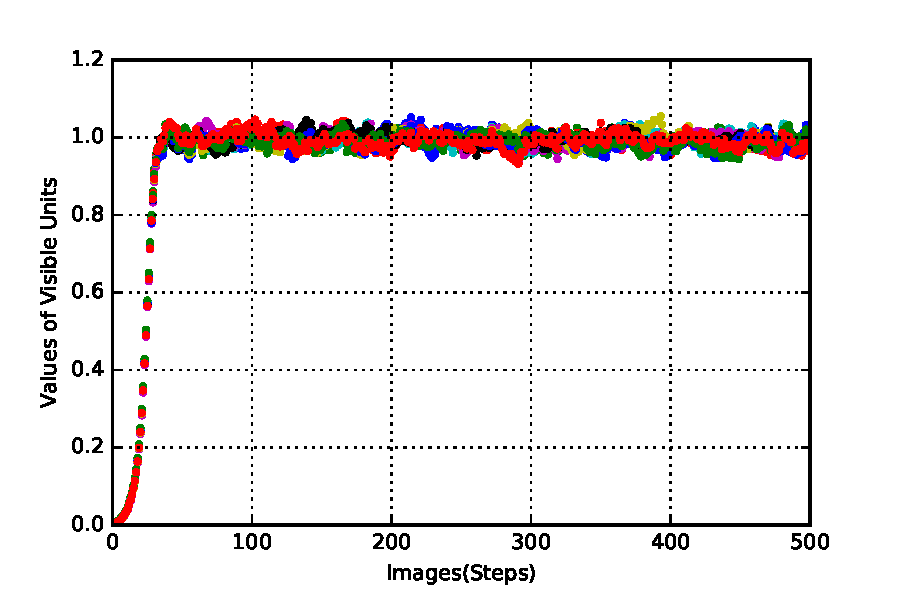
\includegraphics[width=\textwidth]{pics_sdlm/30_exp_RBM/exp1_recon_non.pdf}
		\caption{Reconstruction of visible units in Exp1}
	\end{subfigure}
	\begin{subfigure}[t]{0.4\textwidth}
		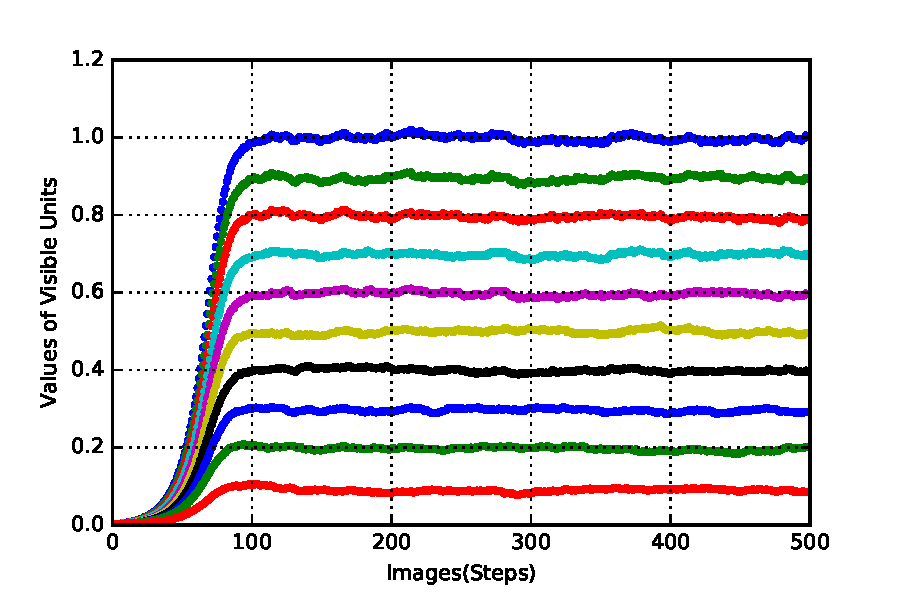
\includegraphics[width=\textwidth]{pics_sdlm/30_exp_RBM/exp2_recon_non.pdf}
		\caption{Reconstruction of visible units in Exp2}
	\end{subfigure}\\
	\begin{subfigure}[t]{0.4\textwidth}
		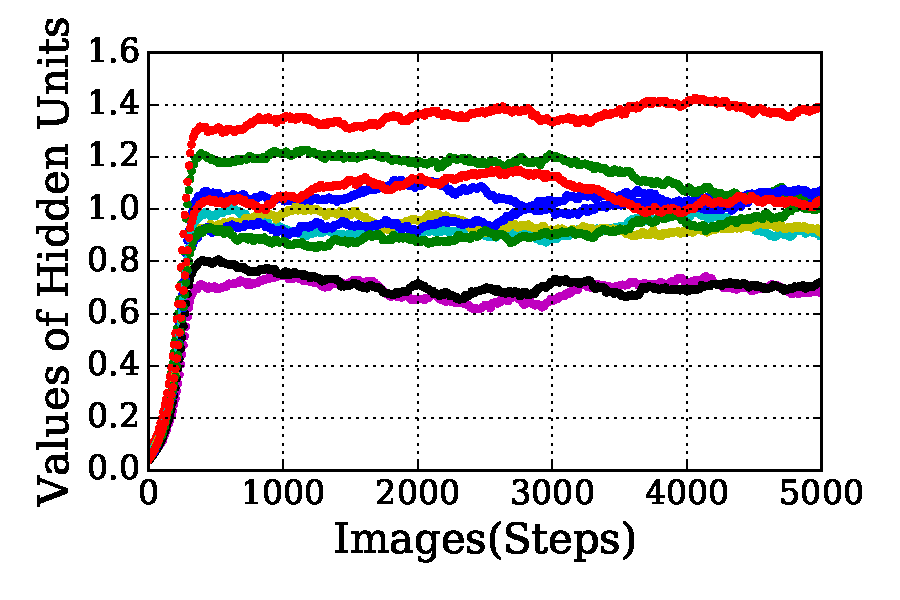
\includegraphics[width=\textwidth]{pics_sdlm/30_exp_RBM/exp1_hid_non.pdf}
		\caption{Output of hidden units in Exp1}
	\end{subfigure}
	\begin{subfigure}[t]{0.4\textwidth}
		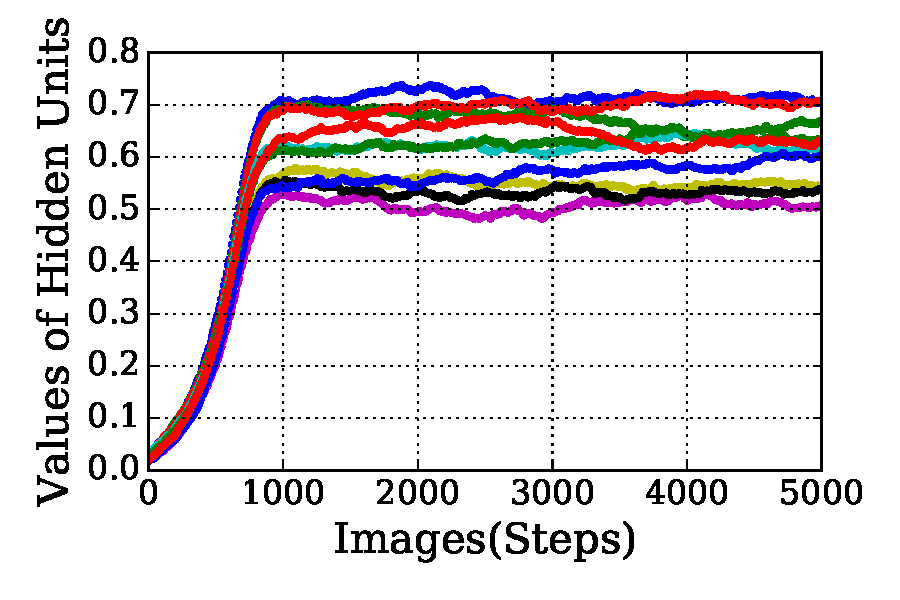
\includegraphics[width=\textwidth]{pics_sdlm/30_exp_RBM/exp2_hid_non.pdf}
		\caption{Output of hidden units in Exp2}
	\end{subfigure}\\
	\begin{subfigure}[t]{0.4\textwidth}
		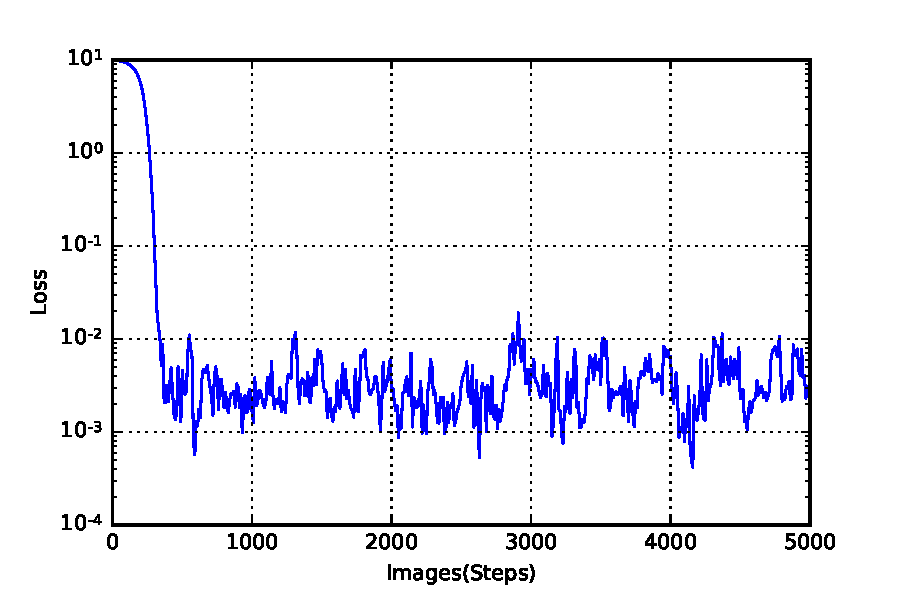
\includegraphics[width=\textwidth]{pics_sdlm/30_exp_RBM/exp1_loss.pdf}
		\caption{Output of hidden units in Exp1}
	\end{subfigure}
	\begin{subfigure}[t]{0.4\textwidth}
		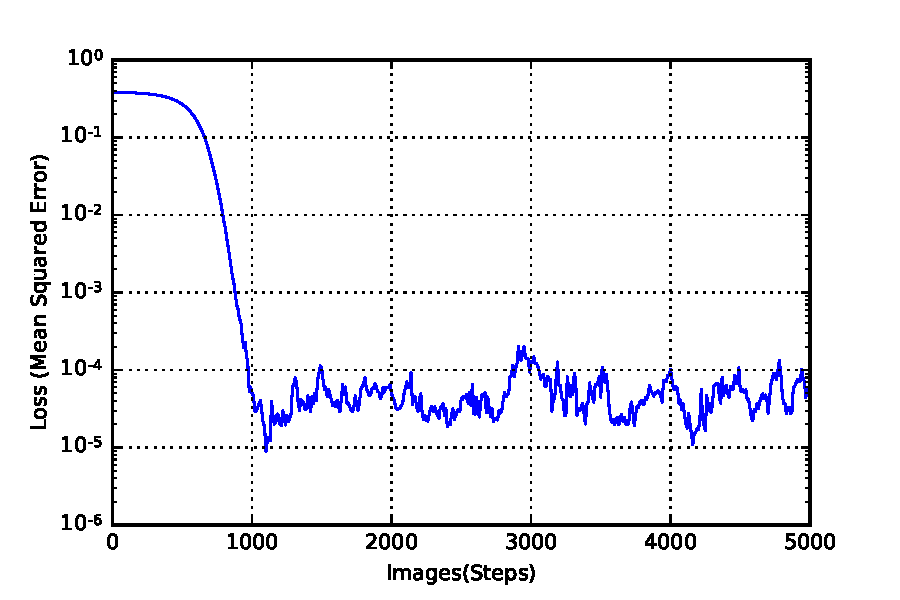
\includegraphics[width=\textwidth]{pics_sdlm/30_exp_RBM/exp2_loss.pdf}
		\caption{Output of hidden units in Exp2}
	\end{subfigure}
	\caption{Changes of weights, output of visible and hidden units, and mean squared error (loss) during the nRBM training of the reconstruction tests. 
		Experiments 1) 10 visible units fully connected to 10 hidden units with input data of all 1s; 2) same network fed with 10 values distribute linearly from 0.1 to 1.}
\end{figure}

\section{Biologically Plausible Training}
\subsection{Rate-based coding}
The encoding method is the same as stated below in Chapter~\ref{sec:poissonian}.
It introduces noise to the original input.
The experiments on noisy input driven by Poissonian spike trains.
Figure~\ref{fig:poisson_ae} and Figure~\ref{fig:poisson_rbm} show how noise influence the training and output of both the visible and hidden units.
The change of the weights oscillates more. % and the value of the weights tends to diverge slightly as training goes on. 
The experiments run as a baseline to compare with spike based training in the following Section.
\begin{figure}
	\centering
	\begin{subfigure}[t]{0.4\textwidth}
		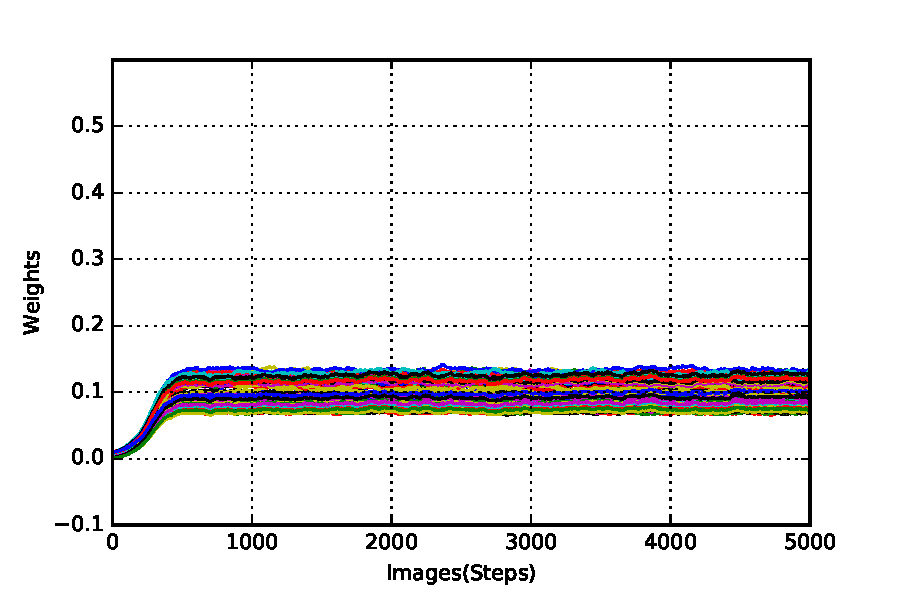
\includegraphics[width=\textwidth]{pics_sdlm/21_exp_AE_noise/exp1_weights_s.pdf}
		\caption{Weights of Exp1}
	\end{subfigure}
	\begin{subfigure}[t]{0.4\textwidth}
		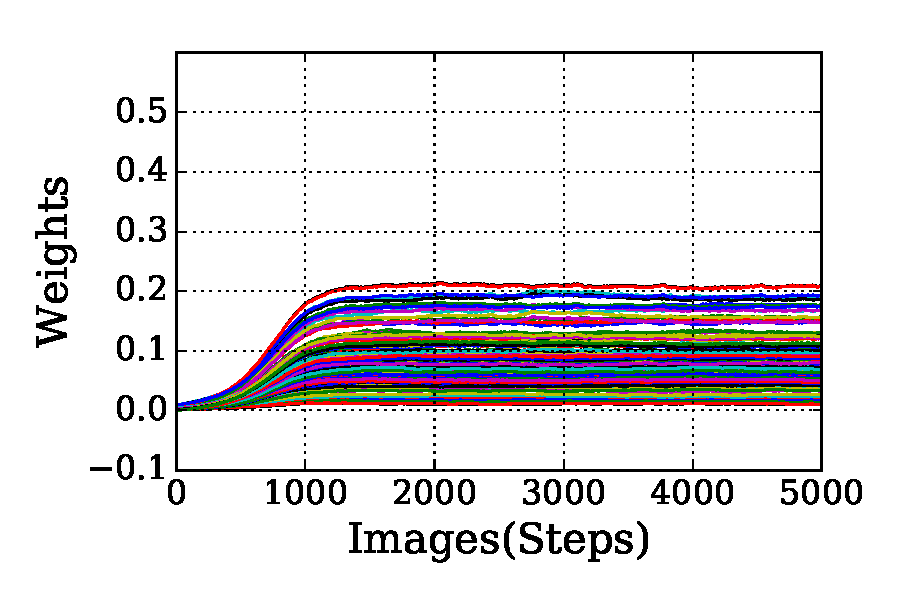
\includegraphics[width=\textwidth]{pics_sdlm/21_exp_AE_noise/exp2_weights_s.pdf}
		\caption{Weights of Exp2}
	\end{subfigure}
	\begin{subfigure}[t]{0.4\textwidth}
		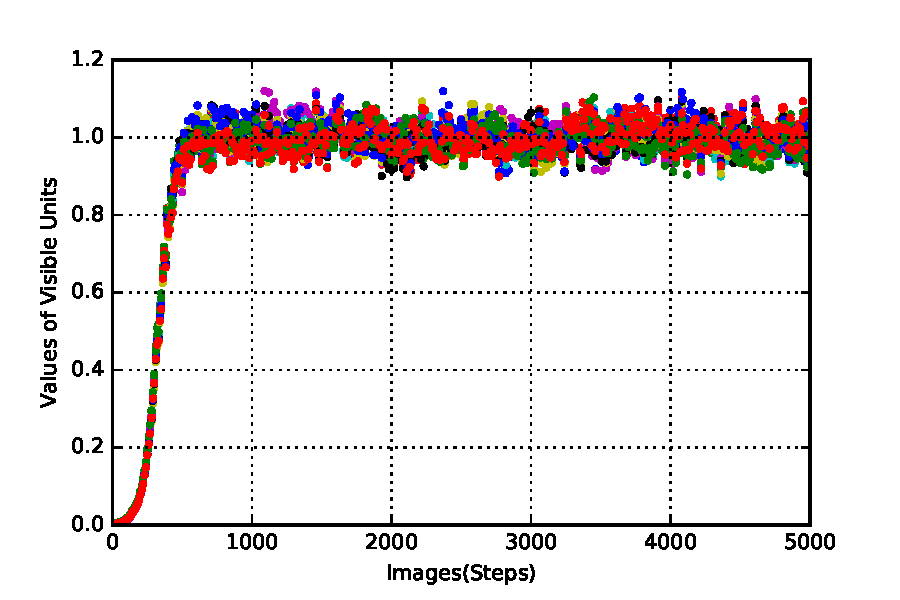
\includegraphics[width=\textwidth]{pics_sdlm/21_exp_AE_noise/exp1_recon_s.pdf}
		\caption{Reconstruction of visible units in Exp1}
	\end{subfigure}
	\begin{subfigure}[t]{0.4\textwidth}
		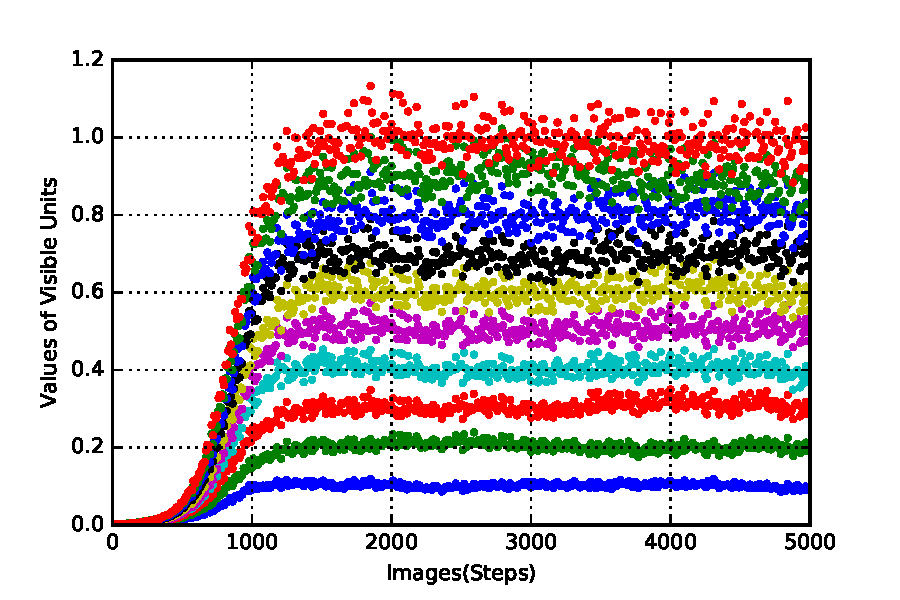
\includegraphics[width=\textwidth]{pics_sdlm/21_exp_AE_noise/exp2_recon_s.pdf}
		\caption{Reconstruction of visible units in Exp2}
	\end{subfigure}\\
	\begin{subfigure}[t]{0.4\textwidth}
		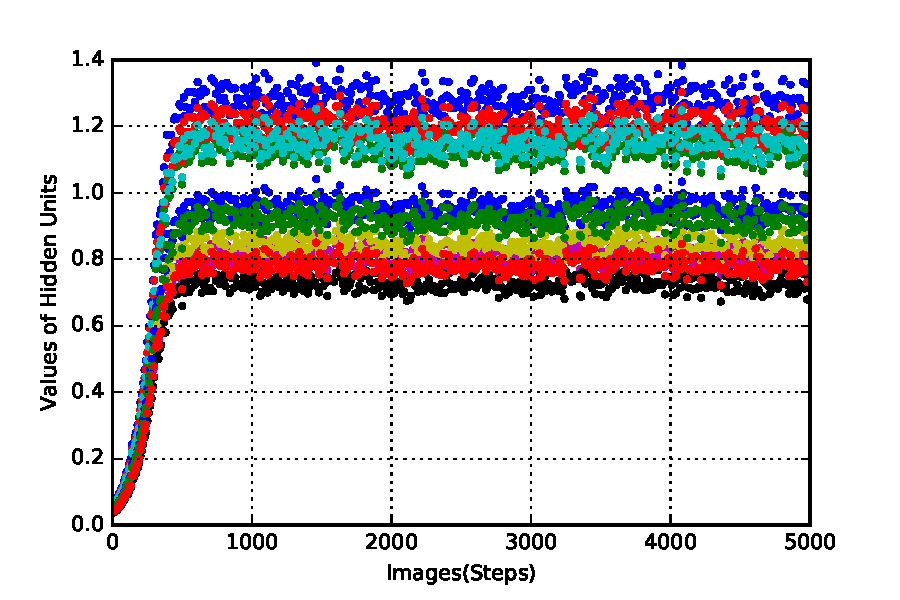
\includegraphics[width=\textwidth]{pics_sdlm/21_exp_AE_noise/exp1_hid_s.pdf}
		\caption{Output of hidden units in Exp1}
	\end{subfigure}
	\begin{subfigure}[t]{0.4\textwidth}
		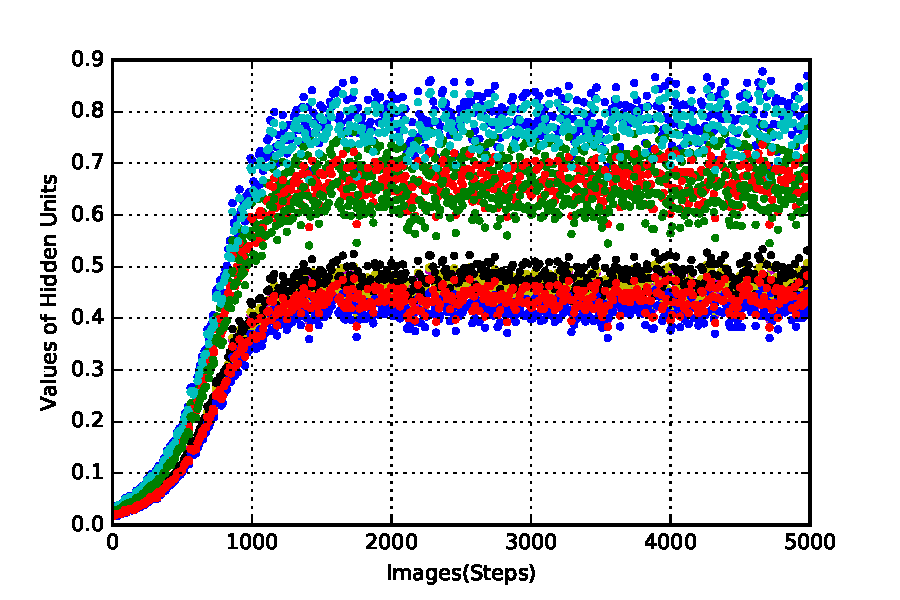
\includegraphics[width=\textwidth]{pics_sdlm/21_exp_AE_noise/exp2_hid_s.pdf}
		\caption{Output of hidden units in Exp2}
	\end{subfigure}\\
	\begin{subfigure}[t]{0.4\textwidth}
		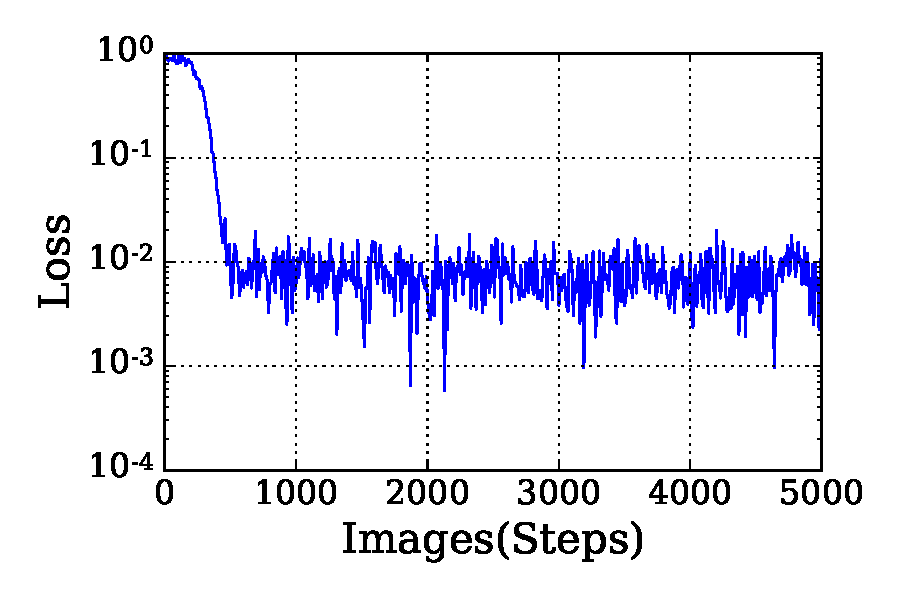
\includegraphics[width=\textwidth]{pics_sdlm/21_exp_AE_noise/exp1_loss_s.pdf}
		\caption{Output of hidden units in Exp1}
	\end{subfigure}
	\begin{subfigure}[t]{0.4\textwidth}
		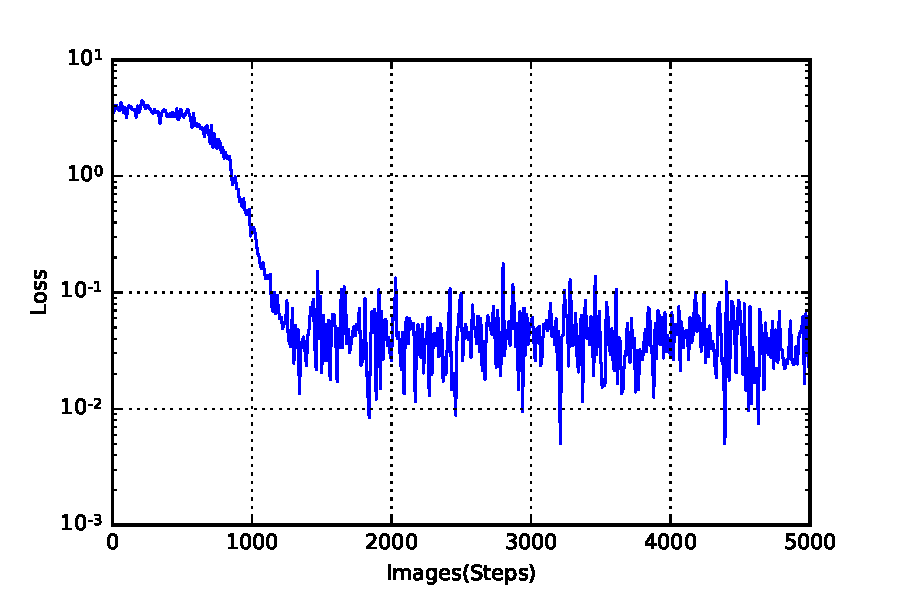
\includegraphics[width=\textwidth]{pics_sdlm/21_exp_AE_noise/exp2_loss_s.pdf}
		\caption{Output of hidden units in Exp2}
	\end{subfigure}
	\caption{Changes of weights, output of visible and hidden units, and mean squared error (loss) during the AE training of the reconstruction tests. 
		Experiments 1) 10 visible units fully connected to 10 hidden units with the count of Poisson spikes firing at 100~Hz which lasted 100~ms; 2) same network fed with 10 count of Poisson spikes at firing rate ranging from 10~Hz to 100~Hz.}
	\label{fig:poisson_ae}
\end{figure}

\begin{figure}
	\centering
	\begin{subfigure}[t]{0.4\textwidth}
		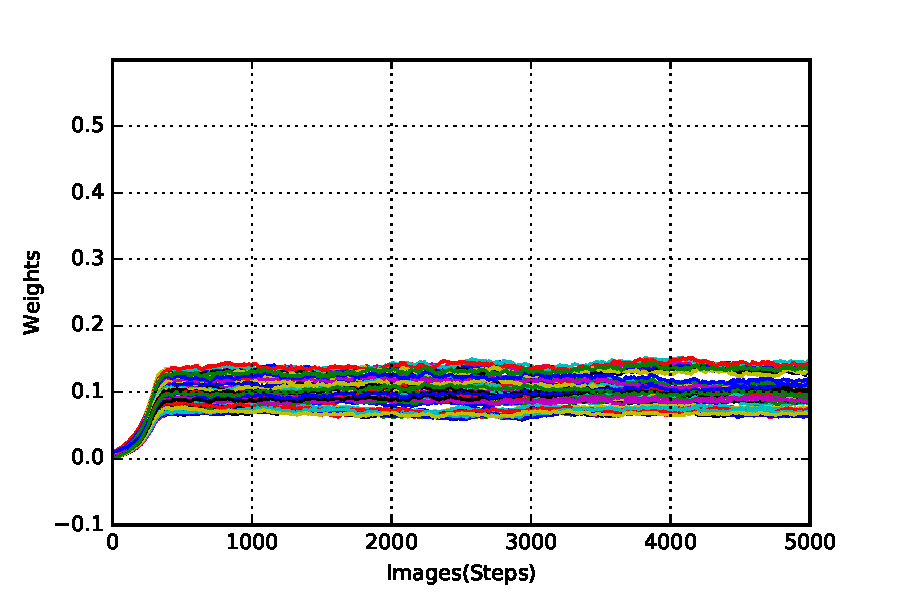
\includegraphics[width=\textwidth]{pics_sdlm/31_exp_RBM_noise/exp1_weights_s.pdf}
		\caption{Weights of Exp1}
	\end{subfigure}
	\begin{subfigure}[t]{0.4\textwidth}
		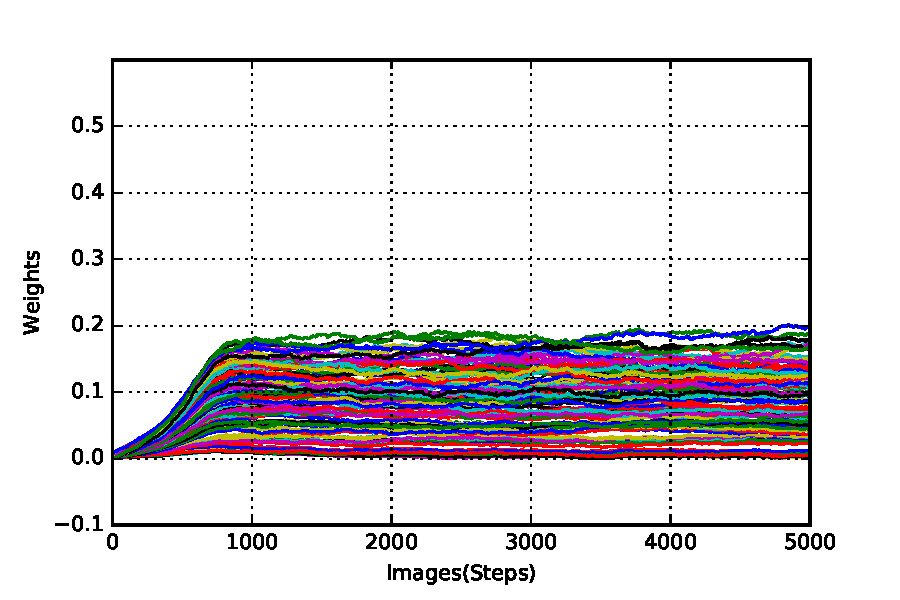
\includegraphics[width=\textwidth]{pics_sdlm/31_exp_RBM_noise/exp2_weights_s.pdf}
		\caption{Weights of Exp2}
	\end{subfigure}
	\begin{subfigure}[t]{0.4\textwidth}
		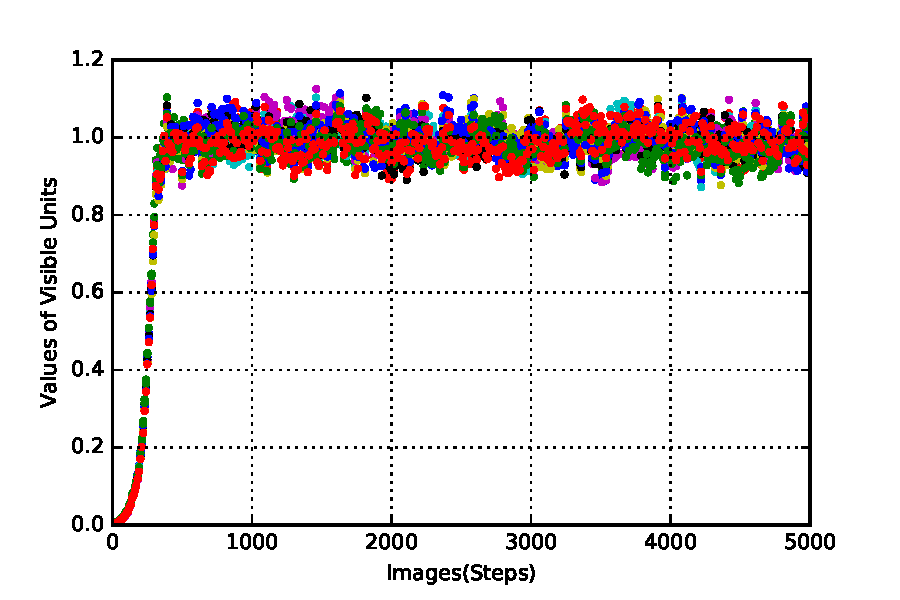
\includegraphics[width=\textwidth]{pics_sdlm/31_exp_RBM_noise/exp1_recon_s.pdf}
		\caption{Reconstruction of visible units in Exp1}
	\end{subfigure}
	\begin{subfigure}[t]{0.4\textwidth}
		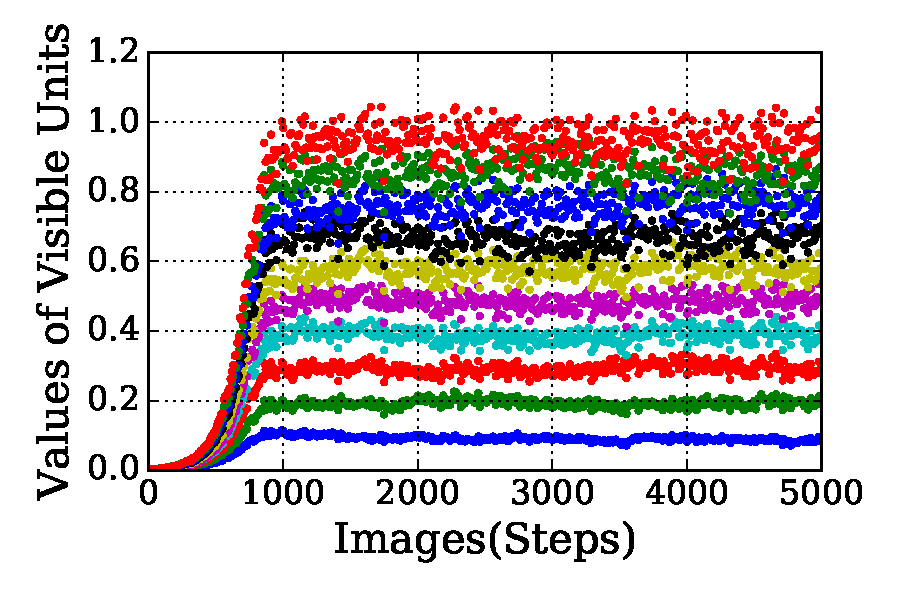
\includegraphics[width=\textwidth]{pics_sdlm/31_exp_RBM_noise/exp2_recon_s.pdf}
		\caption{Reconstruction of visible units in Exp2}
	\end{subfigure}\\
	\begin{subfigure}[t]{0.4\textwidth}
		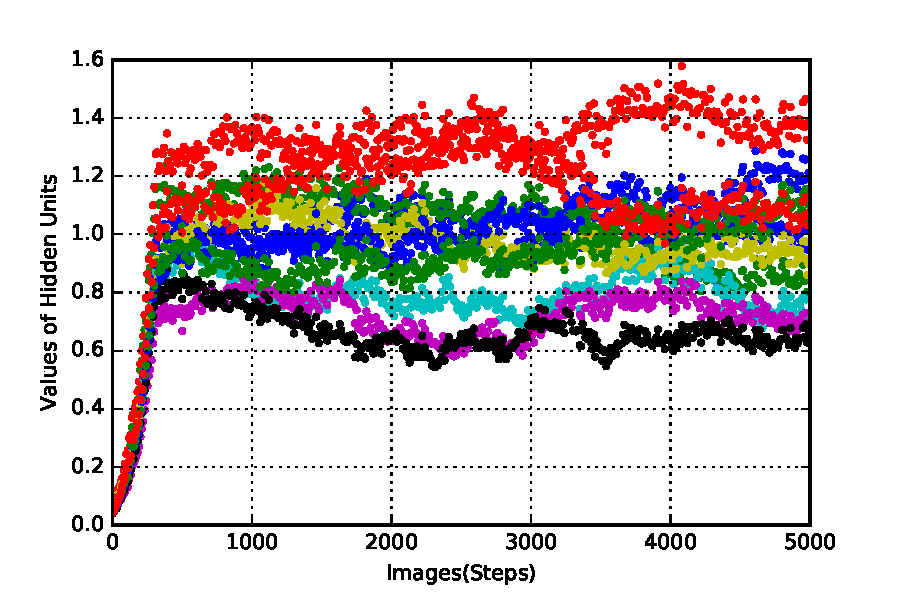
\includegraphics[width=\textwidth]{pics_sdlm/31_exp_RBM_noise/exp1_hid_s.pdf}
		\caption{Output of hidden units in Exp1}
	\end{subfigure}
	\begin{subfigure}[t]{0.4\textwidth}
		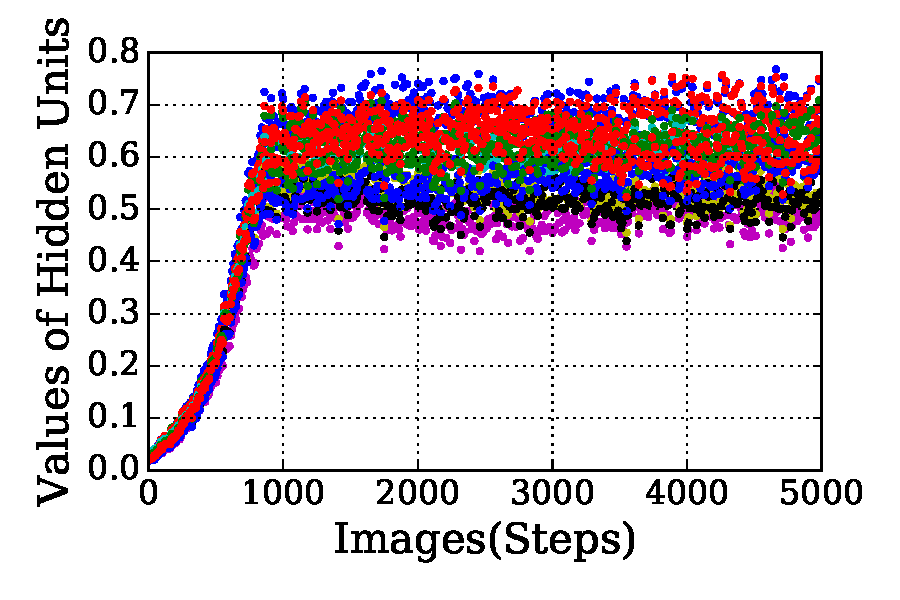
\includegraphics[width=\textwidth]{pics_sdlm/31_exp_RBM_noise/exp2_hid_s.pdf}
		\caption{Output of hidden units in Exp2}
	\end{subfigure}\\
	\begin{subfigure}[t]{0.4\textwidth}
		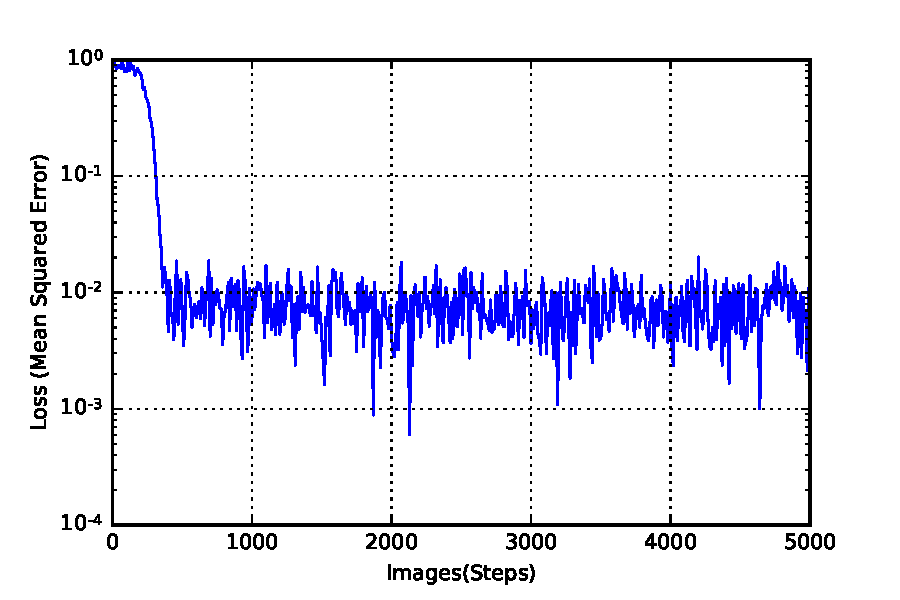
\includegraphics[width=\textwidth]{pics_sdlm/31_exp_RBM_noise/exp1_loss_s.pdf}
		\caption{Output of hidden units in Exp1}
	\end{subfigure}
	\begin{subfigure}[t]{0.4\textwidth}
		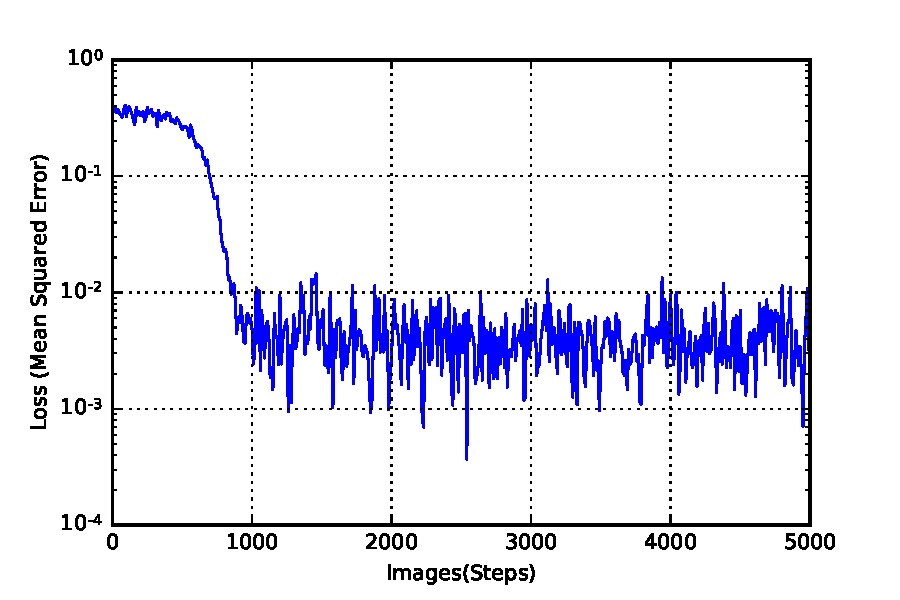
\includegraphics[width=\textwidth]{pics_sdlm/31_exp_RBM_noise/exp2_loss_s.pdf}
		\caption{Output of hidden units in Exp2}
	\end{subfigure}
	\caption{Changes of weights, output of visible and hidden units, and mean squared error (loss) during the nRBM training of the reconstruction tests. 
		Experiments 1) 10 visible units fully connected to 10 hidden units with the count of Poisson spikes firing at 100~Hz which lasted 100~ms; 2) same network fed with 10 count of Poisson spikes at firing rate ranging from 10~Hz to 100~Hz.}
	\label{fig:poisson_rbm}
\end{figure}

\subsection{STDP}

\subsection{Training Spiking Autoencoders}
Rate-based learning of STDP (rSTDP) which is inspired by ReSuMe.
Biology, local\\
-Why it works stated in Maths.\\
\begin{equation}
\begin{aligned}
\overline{\Delta w_{ij}} &\propto \eta \lambda_{h_i}(\lambda_{v_j} - \lambda_{v'_j})\\
&=\eta'P_{h_i}P_{v_j}\tau_{w} \tau_{dur} - \eta'P_{h_i}P_{v'_j}\tau_{w} \tau_{dur}, \textrm{where,}\\
P_{s} &= \lambda_{s} \times 0.001~s = \frac{K s}{1000}\\
\eta' &= \frac{10^6}{K^2 \tau_{w} \tau_{dur}} \eta
\end{aligned}
\end{equation}
\begin{figure}
	\centering
	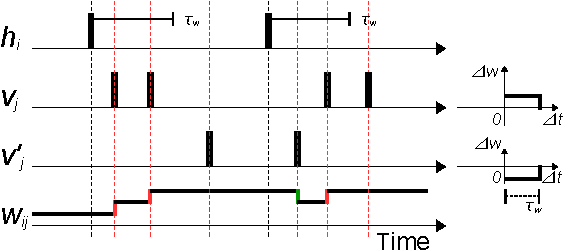
\includegraphics[width=0.8\textwidth]{pics_sdlm/rSTDP.pdf}
	\caption{How rSTDP works in training spiking Autoencoders.}
	\label{fig:rSTDP}
\end{figure}

\subsection{Training Spiking RBM}
\begin{figure}
	\centering
	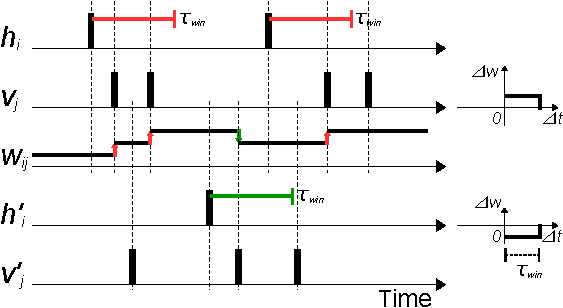
\includegraphics[width=0.8\textwidth]{pics_sdlm/rSTDP_rbm.pdf}
	\caption{How rSTDP works in training spiking RBMs.}
	\label{fig:rSTDP_rbm}
\end{figure}

\section{Problem}
Correlations in spike trains make weights diverge.
Experiments
\begin{figure}
	\centering
	\begin{subfigure}[t]{0.4\textwidth}
		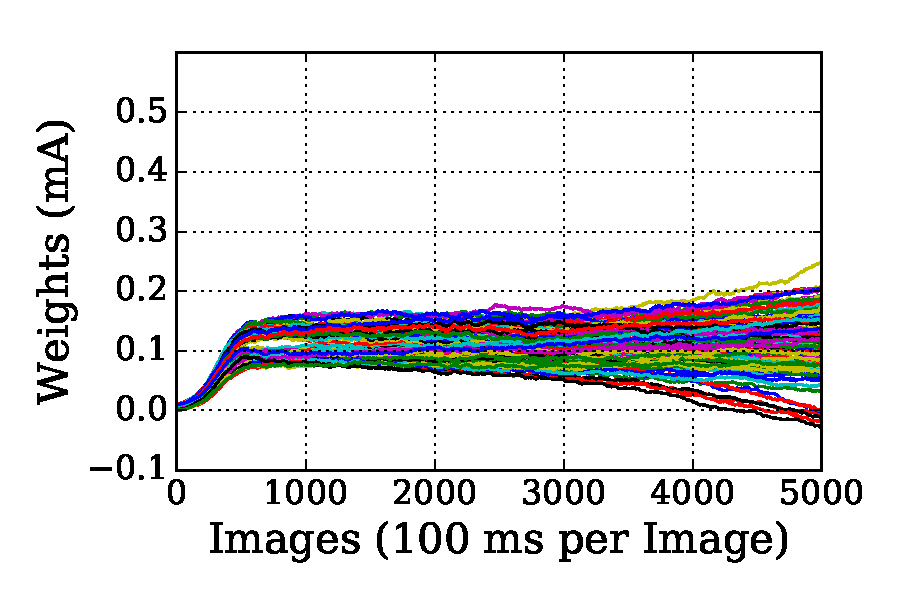
\includegraphics[width=\textwidth]{pics_sdlm/00_exp_SAE_Orig/exp1_weights_s.pdf}
		\caption{Weights of Exp1}
	\end{subfigure}
	\begin{subfigure}[t]{0.4\textwidth}
		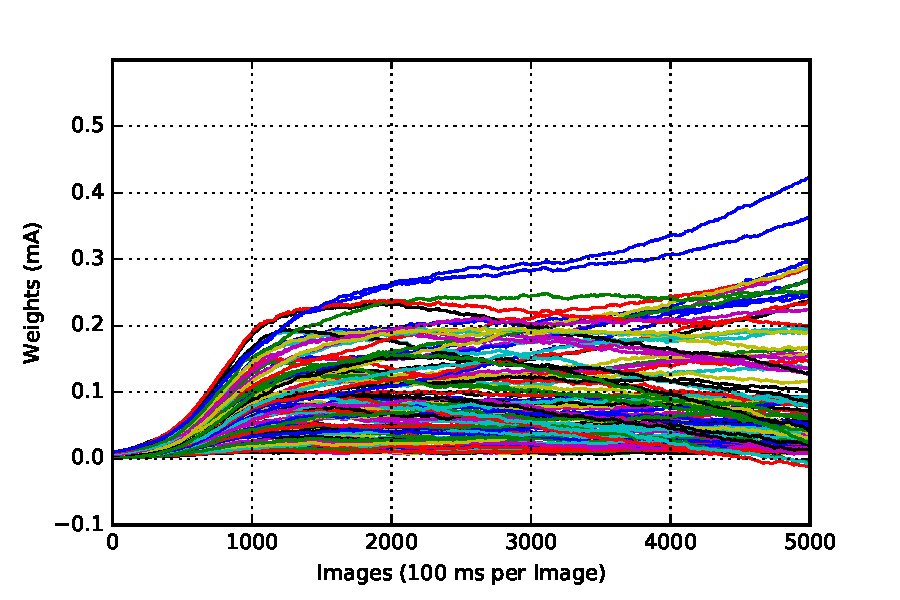
\includegraphics[width=\textwidth]{pics_sdlm/00_exp_SAE_Orig/exp2_weights_s.pdf}
		\caption{Weights of Exp2}
	\end{subfigure}
	\begin{subfigure}[t]{0.4\textwidth}
		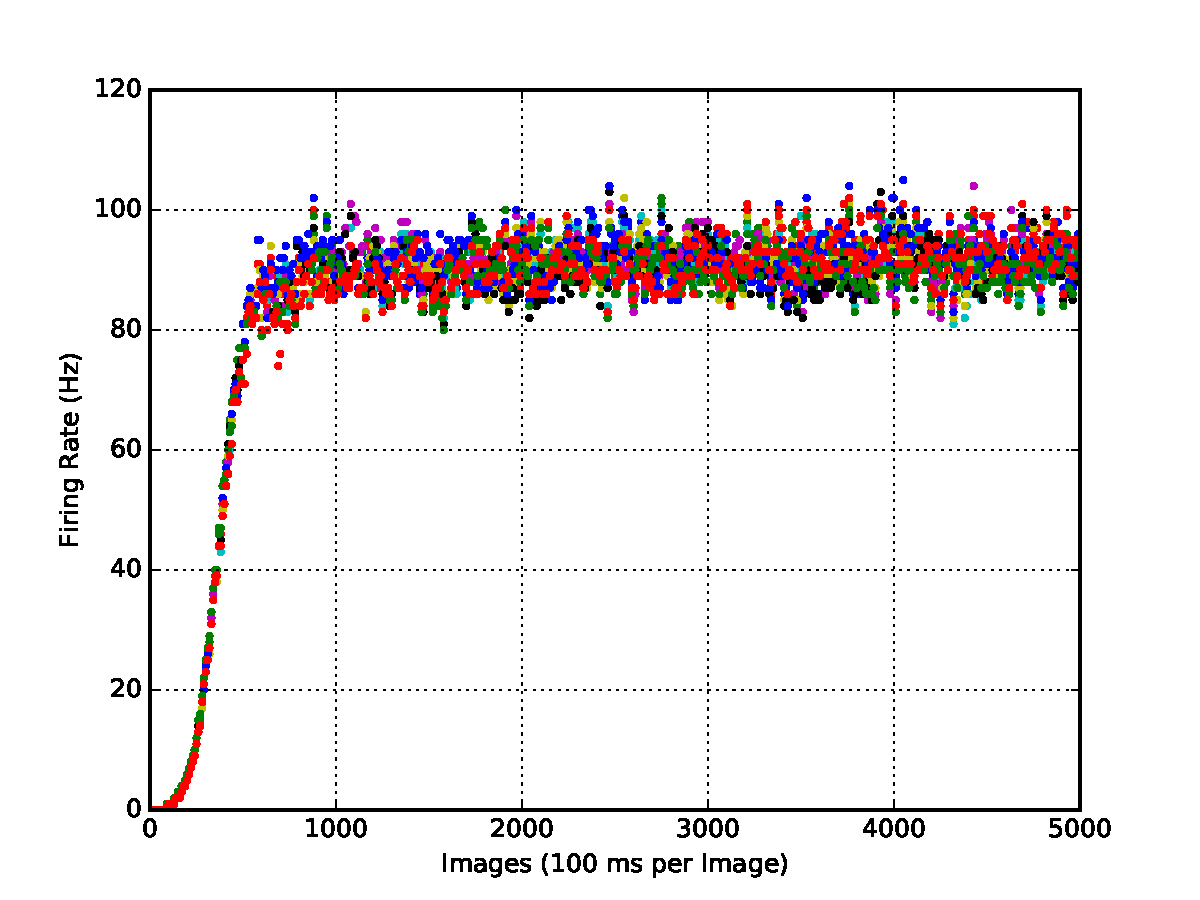
\includegraphics[width=\textwidth]{pics_sdlm/00_exp_SAE_Orig/exp1_recon_s.pdf}
		\caption{Reconstruction of visible units in Exp1}
	\end{subfigure}
	\begin{subfigure}[t]{0.4\textwidth}
		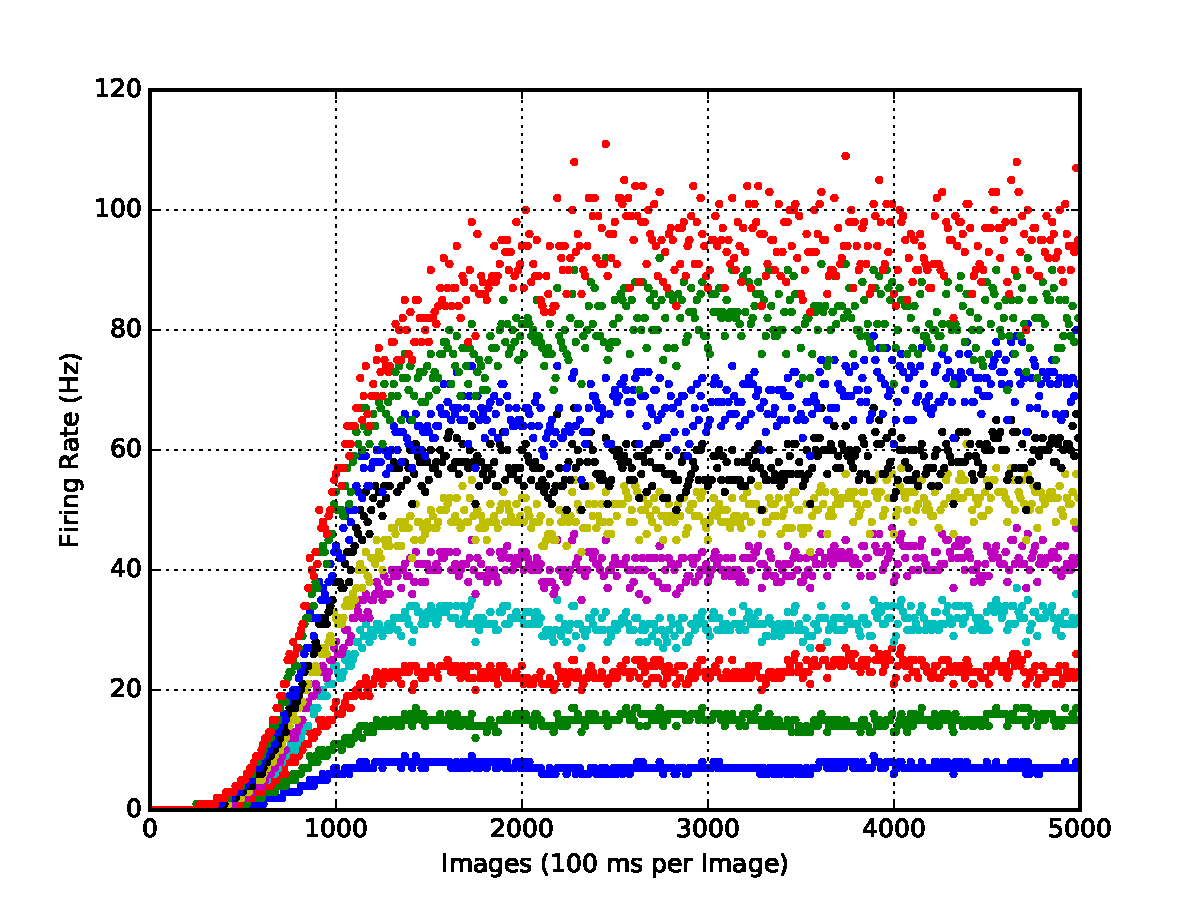
\includegraphics[width=\textwidth]{pics_sdlm/00_exp_SAE_Orig/exp2_recon_s.pdf}
		\caption{Reconstruction of visible units in Exp2}
	\end{subfigure}\\
	\begin{subfigure}[t]{0.4\textwidth}
		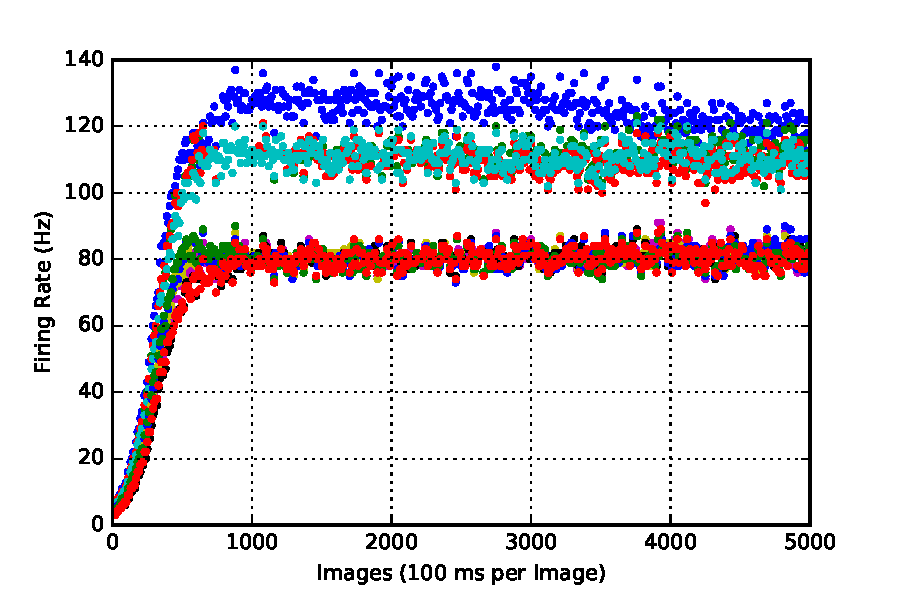
\includegraphics[width=\textwidth]{pics_sdlm/00_exp_SAE_Orig/exp1_hid_s.pdf}
		\caption{Output of hidden units in Exp1}
	\end{subfigure}
	\begin{subfigure}[t]{0.4\textwidth}
		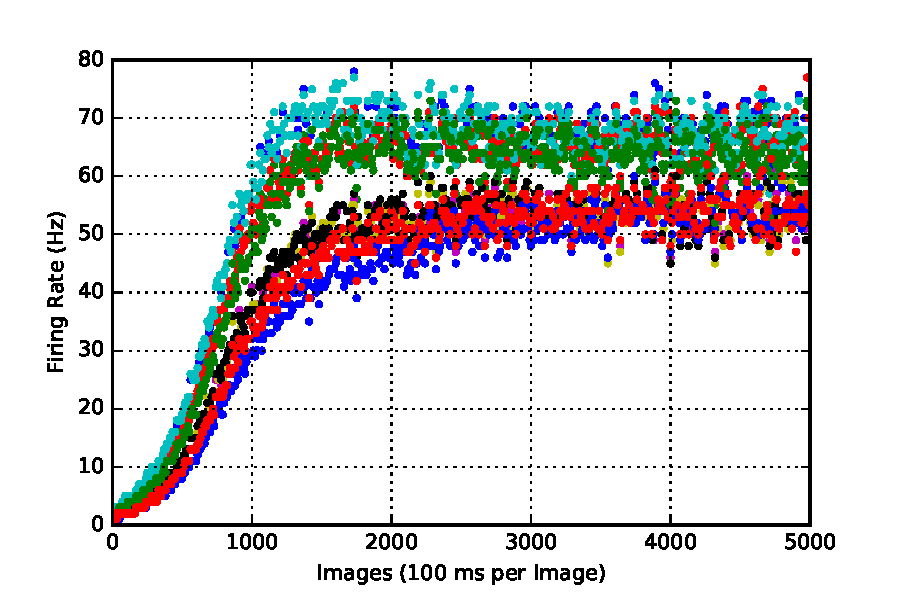
\includegraphics[width=\textwidth]{pics_sdlm/00_exp_SAE_Orig/exp2_hid_s.pdf}
		\caption{Output of hidden units in Exp2}
	\end{subfigure}\\
	\begin{subfigure}[t]{0.4\textwidth}
		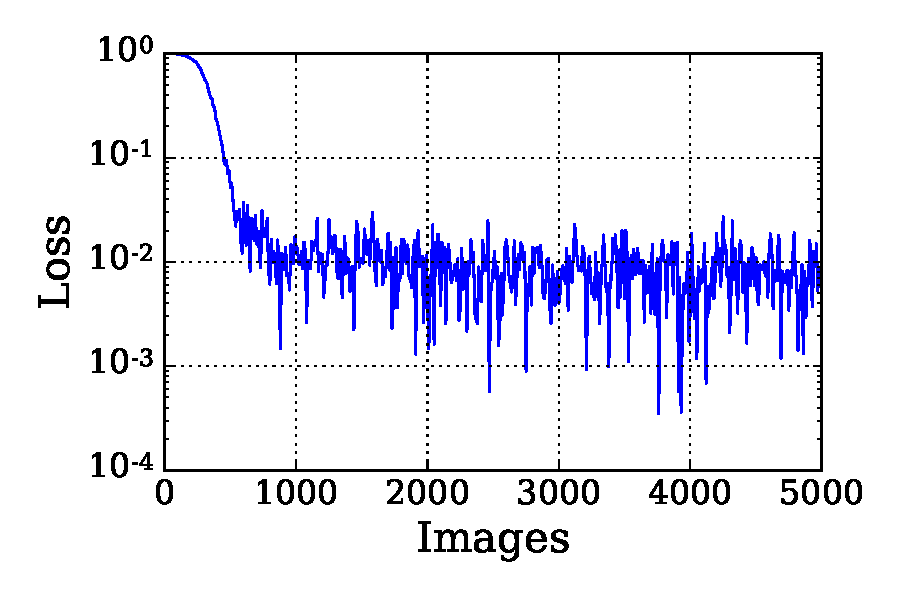
\includegraphics[width=\textwidth]{pics_sdlm/00_exp_SAE_Orig/exp1_mse_nons.pdf}
		\caption{Loss of Exp1}
	\end{subfigure}
	\begin{subfigure}[t]{0.4\textwidth}
		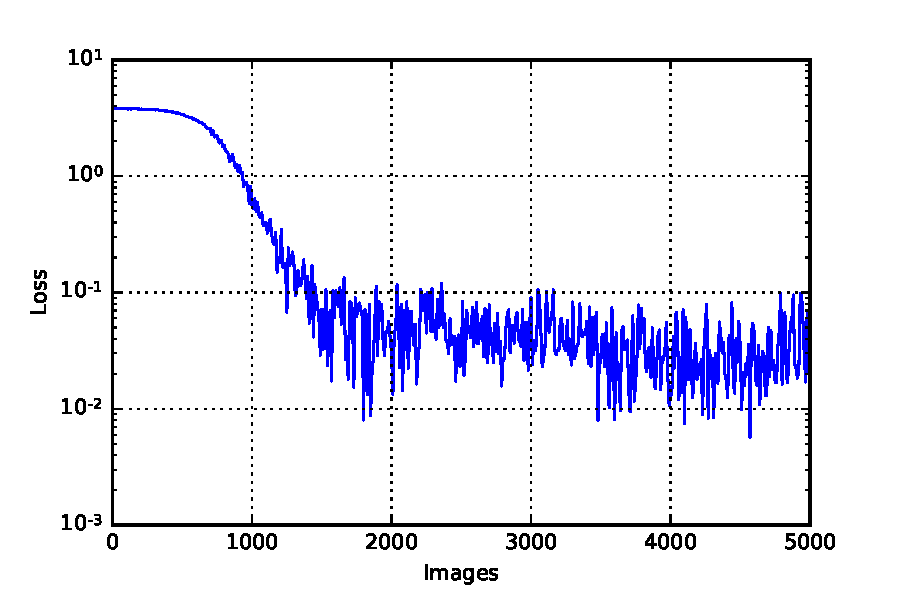
\includegraphics[width=\textwidth]{pics_sdlm/00_exp_SAE_Orig/exp2_mse_nons.pdf}
		\caption{Loss of Exp2}
	\end{subfigure}
	\caption{Weights and firing rates of visible and hidden units change during training of the reconstruction tests of spiking AE. 
		Experiments 1) 10 visible units fully connected to 10 hidden units with Poisson spike trains of 100~Hz which lasted 100~ms; 2) same network fed with 10 Poisson spike trains of firing rate ranging from 10~Hz to 100~Hz.}
\end{figure}

\begin{figure}
	\centering
	\begin{subfigure}[t]{0.4\textwidth}
		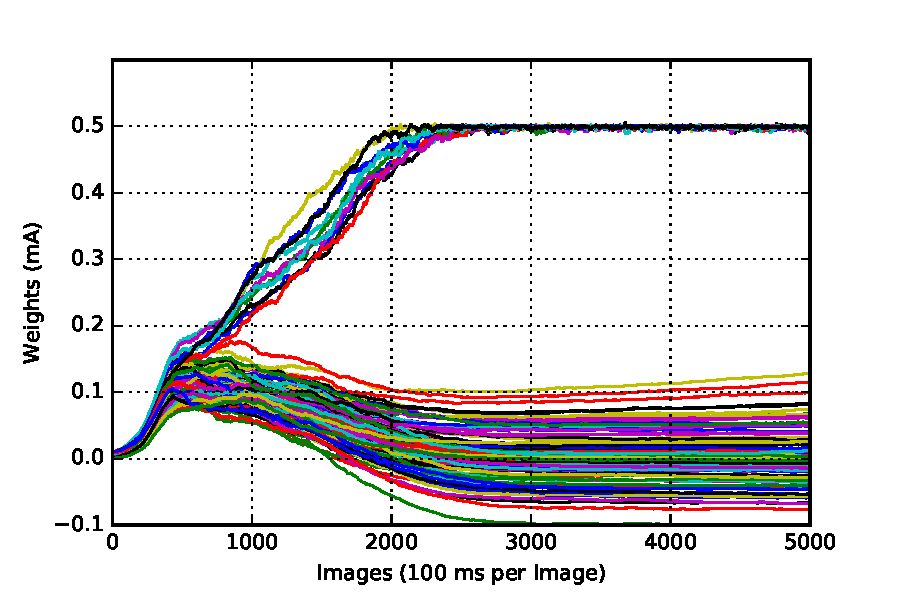
\includegraphics[width=\textwidth]{pics_sdlm/10_exp_SRBM_Orig/exp1_weights_s.pdf}
		\caption{Weights of Exp1}
	\end{subfigure}
	\begin{subfigure}[t]{0.4\textwidth}
		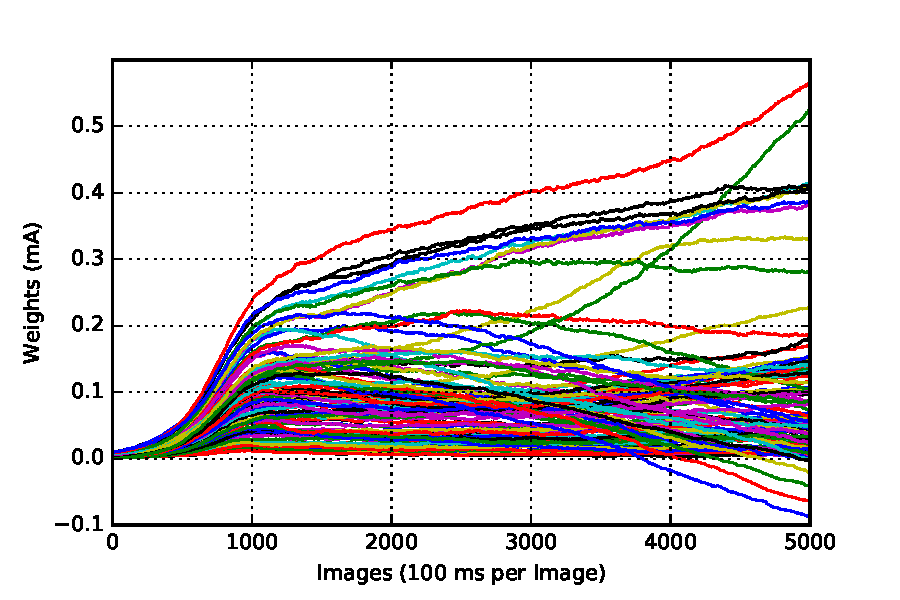
\includegraphics[width=\textwidth]{pics_sdlm/10_exp_SRBM_Orig/exp2_weights_s.pdf}
		\caption{Weights of Exp2}
	\end{subfigure}
	\begin{subfigure}[t]{0.4\textwidth}
		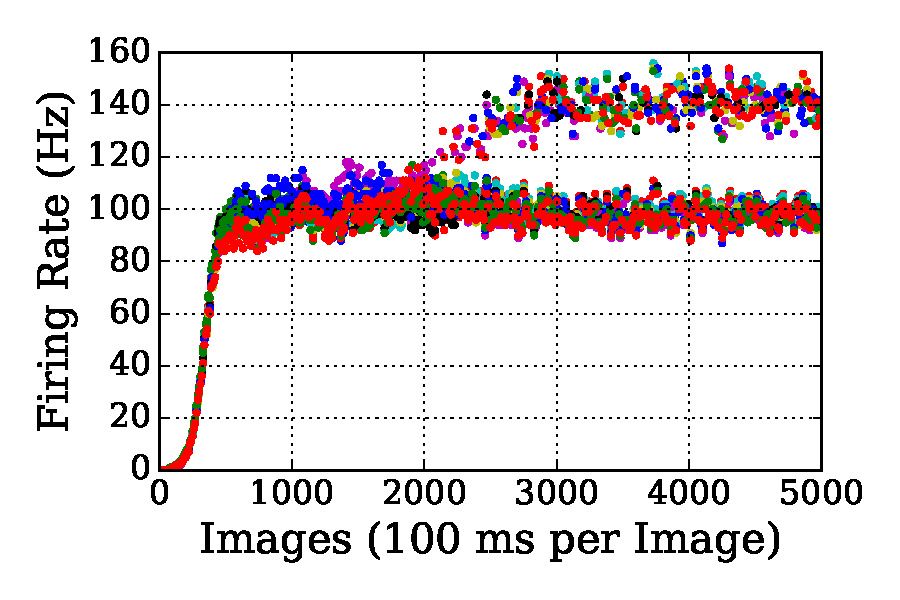
\includegraphics[width=\textwidth]{pics_sdlm/10_exp_SRBM_Orig/exp1_recon_s.pdf}
		\caption{Reconstruction of visible units in Exp1}
	\end{subfigure}
	\begin{subfigure}[t]{0.4\textwidth}
		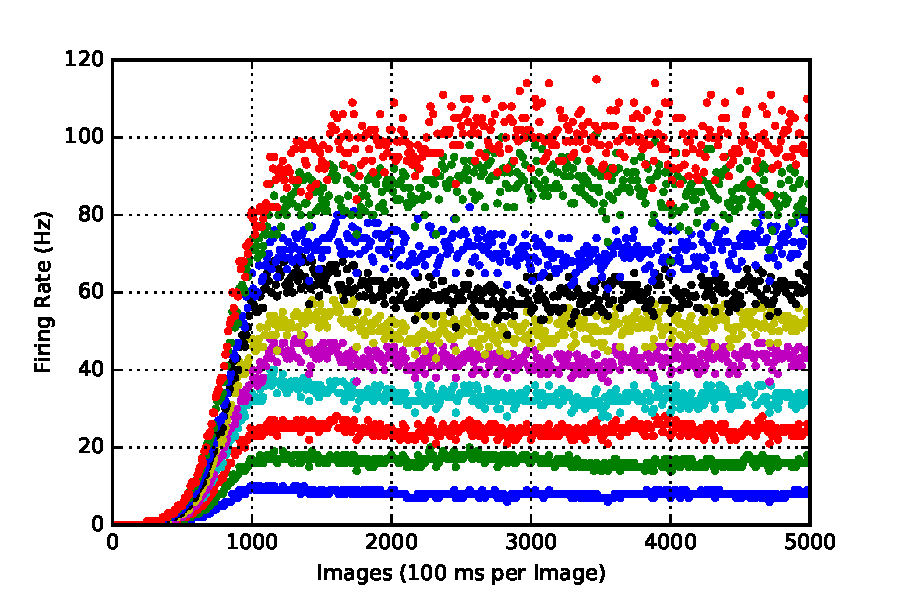
\includegraphics[width=\textwidth]{pics_sdlm/10_exp_SRBM_Orig/exp2_recon_s.pdf}
		\caption{Reconstruction of visible units in Exp2}
	\end{subfigure}\\
	\begin{subfigure}[t]{0.4\textwidth}
		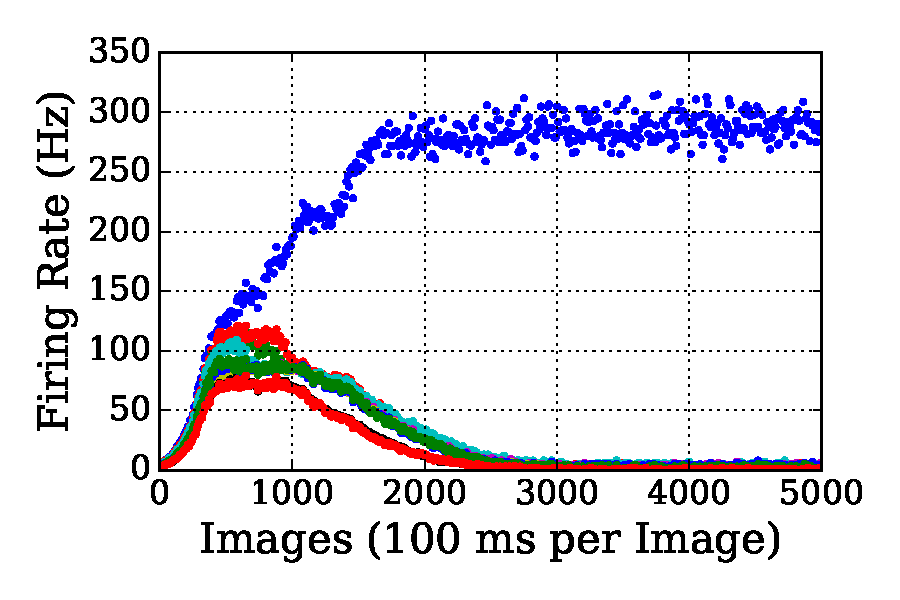
\includegraphics[width=\textwidth]{pics_sdlm/10_exp_SRBM_Orig/exp1_hid_s.pdf}
		\caption{Output of hidden units in Exp1}
	\end{subfigure}
	\begin{subfigure}[t]{0.4\textwidth}
		\includegraphics[width=\textwidth]{pics_sdlm/10_exp_SRBM_Orig/exp2_hid_s.pdf}
		\caption{Output of hidden units in Exp2}
	\end{subfigure}\\
	\begin{subfigure}[t]{0.4\textwidth}
		\includegraphics[width=\textwidth]{pics_sdlm/10_exp_SRBM_Orig/exp1_mse_nons.pdf}
		\caption{Loss of Exp1}
	\end{subfigure}
	\begin{subfigure}[t]{0.4\textwidth}
		\includegraphics[width=\textwidth]{pics_sdlm/10_exp_SRBM_Orig/exp2_mse_nons.pdf}
		\caption{Loss of Exp2}
	\end{subfigure}
	\caption{Weights and firing rates of visible and hidden units change during training of the reconstruction tests of spiking RBM. 
		Experiments 1) 10 visible units fully connected to 10 hidden units with Poisson spike trains of 100~Hz which lasted 100~ms; 2) same network fed with 10 Poisson spike trains of firing rate ranging from 10~Hz to 100~Hz.}
\end{figure}

\subsection{Solution 1: Longer STDP Window}
The stronger correlation of a pair of pre- and post-synaptic neurons make the spikes generated by the post-synaptic neuron lie in the shorter period after the pre-synaptic spike.
So a longer square STDP window maker the overall weight change more dependent of the correlation of the spike trains.
\begin{figure}
	\centering
	\begin{subfigure}[t]{0.4\textwidth}
		\includegraphics[width=\textwidth]{pics_sdlm/01_exp_SAE_Orig_long/exp1_weights_s.pdf}
		\caption{Weights of Exp1}
	\end{subfigure}
	\begin{subfigure}[t]{0.4\textwidth}
		\includegraphics[width=\textwidth]{pics_sdlm/01_exp_SAE_Orig_long/exp2_weights_s.pdf}
		\caption{Weights of Exp2}
	\end{subfigure}
	\begin{subfigure}[t]{0.4\textwidth}
		\includegraphics[width=\textwidth]{pics_sdlm/01_exp_SAE_Orig_long/exp1_recon_s.pdf}
		\caption{Reconstruction of visible units in Exp1}
	\end{subfigure}
	\begin{subfigure}[t]{0.4\textwidth}
		\includegraphics[width=\textwidth]{pics_sdlm/01_exp_SAE_Orig_long/exp2_recon_s.pdf}
		\caption{Reconstruction of visible units in Exp2}
	\end{subfigure}\\
	\begin{subfigure}[t]{0.4\textwidth}
		\includegraphics[width=\textwidth]{pics_sdlm/01_exp_SAE_Orig_long/exp1_hid_s.pdf}
		\caption{Output of hidden units in Exp1}
	\end{subfigure}
	\begin{subfigure}[t]{0.4\textwidth}
		\includegraphics[width=\textwidth]{pics_sdlm/01_exp_SAE_Orig_long/exp2_hid_s.pdf}
		\caption{Output of hidden units in Exp2}
	\end{subfigure}\\
	\begin{subfigure}[t]{0.4\textwidth}
		\includegraphics[width=\textwidth]{pics_sdlm/01_exp_SAE_Orig_long/exp1_mse_nons.pdf}
		\caption{Loss of Exp1}
	\end{subfigure}
	\begin{subfigure}[t]{0.4\textwidth}
		\includegraphics[width=\textwidth]{pics_sdlm/01_exp_SAE_Orig_long/exp2_mse_nons.pdf}
		\caption{Loss of Exp2}
	\end{subfigure}
	\caption{Weights and firing rates of visible and hidden units change during training of the reconstruction tests of spiking AE. 
		Experiments 1) 10 visible units fully connected to 10 hidden units with Poisson spike trains of 100~Hz which lasted 100~ms; 2) same network fed with 10 Poisson spike trains of firing rate ranging from 10~Hz to 100~Hz.}
\end{figure}

\begin{figure}
	\centering
	\begin{subfigure}[t]{0.4\textwidth}
		\includegraphics[width=\textwidth]{pics_sdlm/11_exp_SRBM_Orig_long/exp1_weights_s.pdf}
		\caption{Weights of Exp1}
	\end{subfigure}
	\begin{subfigure}[t]{0.4\textwidth}
		\includegraphics[width=\textwidth]{pics_sdlm/11_exp_SRBM_Orig_long/exp2_weights_s.pdf}
		\caption{Weights of Exp2}
	\end{subfigure}
	\begin{subfigure}[t]{0.4\textwidth}
		\includegraphics[width=\textwidth]{pics_sdlm/11_exp_SRBM_Orig_long/exp1_recon_s.pdf}
		\caption{Reconstruction of visible units in Exp1}
	\end{subfigure}
	\begin{subfigure}[t]{0.4\textwidth}
		\includegraphics[width=\textwidth]{pics_sdlm/11_exp_SRBM_Orig_long/exp2_recon_s.pdf}
		\caption{Reconstruction of visible units in Exp2}
	\end{subfigure}\\
	\begin{subfigure}[t]{0.4\textwidth}
		\includegraphics[width=\textwidth]{pics_sdlm/11_exp_SRBM_Orig_long/exp1_hid_s.pdf}
		\caption{Output of hidden units in Exp1}
	\end{subfigure}
	\begin{subfigure}[t]{0.4\textwidth}
		\includegraphics[width=\textwidth]{pics_sdlm/11_exp_SRBM_Orig_long/exp2_hid_s.pdf}
		\caption{Output of hidden units in Exp2}
	\end{subfigure}\\
	\begin{subfigure}[t]{0.4\textwidth}
		\includegraphics[width=\textwidth]{pics_sdlm/11_exp_SRBM_Orig_long/exp1_mse_nons.pdf}
		\caption{Loss of Exp1}
	\end{subfigure}
	\begin{subfigure}[t]{0.4\textwidth}
		\includegraphics[width=\textwidth]{pics_sdlm/11_exp_SRBM_Orig_long/exp2_mse_nons.pdf}
		\caption{Loss of Exp2}
	\end{subfigure}
	\caption{Weights and firing rates of visible and hidden units change during training of the reconstruction tests of spiking RBM. 
		Experiments 1) 10 visible units fully connected to 10 hidden units with Poisson spike trains of 100~Hz which lasted 100~ms; 2) same network fed with 10 Poisson spike trains of firing rate ranging from 10~Hz to 100~Hz.}
\end{figure}
\subsection{Solution 2: Noisy Threshold}
There are various ways to introduce noise in formal spiking neuron models. In this section we focus on a `noisy threshold' (also called escape or hazard model)~\cite{gerstner2002spiking}.
The noise drives the post-synaptic spikes fire in advance or behind the expected time, thus it reduces the correlation between the pre- and post synaptic spikes.

\begin{figure}
	\centering
	\begin{subfigure}[t]{0.4\textwidth}
		\includegraphics[width=\textwidth]{pics_sdlm/03_exp_SAE_noise_long/exp1_weights_s.pdf}
		\caption{Weights of Exp1}
	\end{subfigure}
	\begin{subfigure}[t]{0.4\textwidth}
		\includegraphics[width=\textwidth]{pics_sdlm/03_exp_SAE_noise_long/exp2_weights_s.pdf}
		\caption{Weights of Exp2}
	\end{subfigure}
	\begin{subfigure}[t]{0.4\textwidth}
		\includegraphics[width=\textwidth]{pics_sdlm/03_exp_SAE_noise_long/exp1_recon_s.pdf}
		\caption{Reconstruction of visible units in Exp1}
	\end{subfigure}
	\begin{subfigure}[t]{0.4\textwidth}
		\includegraphics[width=\textwidth]{pics_sdlm/03_exp_SAE_noise_long/exp2_recon_s.pdf}
		\caption{Reconstruction of visible units in Exp2}
	\end{subfigure}\\
	\begin{subfigure}[t]{0.4\textwidth}
		\includegraphics[width=\textwidth]{pics_sdlm/03_exp_SAE_noise_long/exp1_hid_s.pdf}
		\caption{Output of hidden units in Exp1}
	\end{subfigure}
	\begin{subfigure}[t]{0.4\textwidth}
		\includegraphics[width=\textwidth]{pics_sdlm/03_exp_SAE_noise_long/exp2_hid_s.pdf}
		\caption{Output of hidden units in Exp2}
	\end{subfigure}\\
	\begin{subfigure}[t]{0.4\textwidth}
		\includegraphics[width=\textwidth]{pics_sdlm/03_exp_SAE_noise_long/exp1_mse_nons.pdf}
		\caption{Loss of Exp1}
	\end{subfigure}
	\begin{subfigure}[t]{0.4\textwidth}
		\includegraphics[width=\textwidth]{pics_sdlm/03_exp_SAE_noise_long/exp2_mse_nons.pdf}
		\caption{Loss of Exp2}
	\end{subfigure}
	\caption{Weights and firing rates of visible and hidden units change during training of the reconstruction tests of spiking AE. 
		Experiments 1) 10 visible units fully connected to 10 hidden units with Poisson spike trains of 100~Hz which lasted 100~ms; 2) same network fed with 10 Poisson spike trains of firing rate ranging from 10~Hz to 100~Hz.}
\end{figure}

\begin{figure}
	\centering
	\begin{subfigure}[t]{0.4\textwidth}
		\includegraphics[width=\textwidth]{pics_sdlm/13_exp_SRBM_noise_long/exp1_weights_s.pdf}
		\caption{Weights of Exp1}
	\end{subfigure}
	\begin{subfigure}[t]{0.4\textwidth}
		\includegraphics[width=\textwidth]{pics_sdlm/13_exp_SRBM_noise_long/exp2_weights_s.pdf}
		\caption{Weights of Exp2}
	\end{subfigure}
	\begin{subfigure}[t]{0.4\textwidth}
		\includegraphics[width=\textwidth]{pics_sdlm/13_exp_SRBM_noise_long/exp1_recon_s.pdf}
		\caption{Reconstruction of visible units in Exp1}
	\end{subfigure}
	\begin{subfigure}[t]{0.4\textwidth}
		\includegraphics[width=\textwidth]{pics_sdlm/13_exp_SRBM_noise_long/exp2_recon_s.pdf}
		\caption{Reconstruction of visible units in Exp2}
	\end{subfigure}\\
	\begin{subfigure}[t]{0.4\textwidth}
		\includegraphics[width=\textwidth]{pics_sdlm/13_exp_SRBM_noise_long/exp1_hid_s.pdf}
		\caption{Output of hidden units in Exp1}
	\end{subfigure}
	\begin{subfigure}[t]{0.4\textwidth}
		\includegraphics[width=\textwidth]{pics_sdlm/13_exp_SRBM_noise_long/exp2_hid_s.pdf}
		\caption{Output of hidden units in Exp2}
	\end{subfigure}\\
	\begin{subfigure}[t]{0.4\textwidth}
		\includegraphics[width=\textwidth]{pics_sdlm/13_exp_SRBM_noise_long/exp1_mse_nons.pdf}
		\caption{Loss of Exp1}
	\end{subfigure}
	\begin{subfigure}[t]{0.4\textwidth}
		\includegraphics[width=\textwidth]{pics_sdlm/13_exp_SRBM_noise_long/exp2_mse_nons.pdf}
		\caption{Loss of Exp2}
	\end{subfigure}
	\caption{Weights and firing rates of visible and hidden units change during training of the reconstruction tests of spiking RBM. 
		Experiments 1) 10 visible units fully connected to 10 hidden units with Poisson spike trains of 100~Hz which lasted 100~ms; 2) same network fed with 10 Poisson spike trains of firing rate ranging from 10~Hz to 100~Hz.}
\end{figure}


\subsection{Solution 3: Teaching Signal}
Teaching spike train firing at the same rate with input spikes is completely decorrelated with the spikes generated in the network.
Thus it decorrelates the positive part of the weight change (red bar in Figure~\ref{fig:rSTDP} and~\ref{fig:rSTDP_rbm}).
\begin{figure}
	\centering
	\begin{subfigure}[t]{0.4\textwidth}
		\includegraphics[width=\textwidth]{pics_sdlm/05_exp_SAE_teach_long/exp1_weights_s.pdf}
		\caption{Weights of Exp1}
	\end{subfigure}
	\begin{subfigure}[t]{0.4\textwidth}
		\includegraphics[width=\textwidth]{pics_sdlm/05_exp_SAE_teach_long/exp2_weights_s.pdf}
		\caption{Weights of Exp2}
	\end{subfigure}
	\begin{subfigure}[t]{0.4\textwidth}
		\includegraphics[width=\textwidth]{pics_sdlm/05_exp_SAE_teach_long/exp1_recon_s.pdf}
		\caption{Reconstruction of visible units in Exp1}
	\end{subfigure}
	\begin{subfigure}[t]{0.4\textwidth}
		\includegraphics[width=\textwidth]{pics_sdlm/05_exp_SAE_teach_long/exp2_recon_s.pdf}
		\caption{Reconstruction of visible units in Exp2}
	\end{subfigure}\\
	\begin{subfigure}[t]{0.4\textwidth}
		\includegraphics[width=\textwidth]{pics_sdlm/05_exp_SAE_teach_long/exp1_hid_s.pdf}
		\caption{Output of hidden units in Exp1}
	\end{subfigure}
	\begin{subfigure}[t]{0.4\textwidth}
		\includegraphics[width=\textwidth]{pics_sdlm/05_exp_SAE_teach_long/exp2_hid_s.pdf}
		\caption{Output of hidden units in Exp2}
	\end{subfigure}\\
	\begin{subfigure}[t]{0.4\textwidth}
		\includegraphics[width=\textwidth]{pics_sdlm/05_exp_SAE_teach_long/exp1_mse_nons.pdf}
		\caption{Loss of Exp1}
	\end{subfigure}
	\begin{subfigure}[t]{0.4\textwidth}
		\includegraphics[width=\textwidth]{pics_sdlm/05_exp_SAE_teach_long/exp2_mse_nons.pdf}
		\caption{Loss of Exp2}
	\end{subfigure}
	\caption{Weights and firing rates of visible and hidden units change during training of the reconstruction tests of spiking AE. 
		Experiments 1) 10 visible units fully connected to 10 hidden units with Poisson spike trains of 100~Hz which lasted 100~ms; 2) same network fed with 10 Poisson spike trains of firing rate ranging from 10~Hz to 100~Hz.}
\end{figure}

\begin{figure}
	\centering
	\begin{subfigure}[t]{0.4\textwidth}
		\includegraphics[width=\textwidth]{pics_sdlm/15_exp_SRBM_teach_long/exp1_weights_s.pdf}
		\caption{Weights of Exp1}
	\end{subfigure}
	\begin{subfigure}[t]{0.4\textwidth}
		\includegraphics[width=\textwidth]{pics_sdlm/15_exp_SRBM_teach_long/exp2_weights_s.pdf}
		\caption{Weights of Exp2}
	\end{subfigure}
	\begin{subfigure}[t]{0.4\textwidth}
		\includegraphics[width=\textwidth]{pics_sdlm/15_exp_SRBM_teach_long/exp1_recon_s.pdf}
		\caption{Reconstruction of visible units in Exp1}
	\end{subfigure}
	\begin{subfigure}[t]{0.4\textwidth}
		\includegraphics[width=\textwidth]{pics_sdlm/15_exp_SRBM_teach_long/exp2_recon_s.pdf}
		\caption{Reconstruction of visible units in Exp2}
	\end{subfigure}\\
	\begin{subfigure}[t]{0.4\textwidth}
		\includegraphics[width=\textwidth]{pics_sdlm/15_exp_SRBM_teach_long/exp1_hid_s.pdf}
		\caption{Output of hidden units in Exp1}
	\end{subfigure}
	\begin{subfigure}[t]{0.4\textwidth}
		\includegraphics[width=\textwidth]{pics_sdlm/15_exp_SRBM_teach_long/exp2_hid_s.pdf}
		\caption{Output of hidden units in Exp2}
	\end{subfigure}\\
	\begin{subfigure}[t]{0.4\textwidth}
		\includegraphics[width=\textwidth]{pics_sdlm/15_exp_SRBM_teach_long/exp1_mse_nons.pdf}
		\caption{Loss of Exp1}
	\end{subfigure}
	\begin{subfigure}[t]{0.4\textwidth}
		\includegraphics[width=\textwidth]{pics_sdlm/15_exp_SRBM_teach_long/exp2_mse_nons.pdf}
		\caption{Loss of Exp2}
	\end{subfigure}
	\caption{Weights and firing rates of visible and hidden units change during training of the reconstruction tests of spiking RBM. 
		Experiments 1) 10 visible units fully connected to 10 hidden units with Poisson spike trains of 100~Hz which lasted 100~ms; 2) same network fed with 10 Poisson spike trains of firing rate ranging from 10~Hz to 100~Hz.}
\end{figure}

\subsection{Test on Combined Solutions}
Same test:
\begin{figure}
	\centering
	\begin{subfigure}[t]{0.4\textwidth}
		\includegraphics[width=\textwidth]{pics_sdlm/07_exp_SAE_all_long/exp1_weights_s.pdf}
		\caption{Weights of Exp1}
	\end{subfigure}
	\begin{subfigure}[t]{0.4\textwidth}
		\includegraphics[width=\textwidth]{pics_sdlm/07_exp_SAE_all_long/exp2_weights_s.pdf}
		\caption{Weights of Exp2}
	\end{subfigure}
	\begin{subfigure}[t]{0.4\textwidth}
		\includegraphics[width=\textwidth]{pics_sdlm/07_exp_SAE_all_long/exp1_recon_s.pdf}
		\caption{Reconstruction of visible units in Exp1}
	\end{subfigure}
	\begin{subfigure}[t]{0.4\textwidth}
		\includegraphics[width=\textwidth]{pics_sdlm/07_exp_SAE_all_long/exp2_recon_s.pdf}
		\caption{Reconstruction of visible units in Exp2}
	\end{subfigure}\\
	\begin{subfigure}[t]{0.4\textwidth}
		\includegraphics[width=\textwidth]{pics_sdlm/07_exp_SAE_all_long/exp1_hid_s.pdf}
		\caption{Output of hidden units in Exp1}
	\end{subfigure}
	\begin{subfigure}[t]{0.4\textwidth}
		\includegraphics[width=\textwidth]{pics_sdlm/07_exp_SAE_all_long/exp2_hid_s.pdf}
		\caption{Output of hidden units in Exp2}
	\end{subfigure}\\
	\begin{subfigure}[t]{0.4\textwidth}
		\includegraphics[width=\textwidth]{pics_sdlm/07_exp_SAE_all_long/exp1_mse_nons.pdf}
		\caption{Loss of Exp1}
	\end{subfigure}
	\begin{subfigure}[t]{0.4\textwidth}
		\includegraphics[width=\textwidth]{pics_sdlm/07_exp_SAE_all_long/exp2_mse_nons.pdf}
		\caption{Loss of Exp2}
	\end{subfigure}
	\caption{Weights and firing rates of visible and hidden units change during training of the reconstruction tests of spiking AE. 
		Experiments 1) 10 visible units fully connected to 10 hidden units with Poisson spike trains of 100~Hz which lasted 100~ms; 2) same network fed with 10 Poisson spike trains of firing rate ranging from 10~Hz to 100~Hz.}
\end{figure}

\begin{figure}
	\centering
	\begin{subfigure}[t]{0.4\textwidth}
		\includegraphics[width=\textwidth]{pics_sdlm/17_exp_SRBM_all_long/exp1_weights_s.pdf}
		\caption{Weights of Exp1}
	\end{subfigure}
	\begin{subfigure}[t]{0.4\textwidth}
		\includegraphics[width=\textwidth]{pics_sdlm/17_exp_SRBM_all_long/exp2_weights_s.pdf}
		\caption{Weights of Exp2}
	\end{subfigure}
	\begin{subfigure}[t]{0.4\textwidth}
		\includegraphics[width=\textwidth]{pics_sdlm/17_exp_SRBM_all_long/exp1_recon_s.pdf}
		\caption{Reconstruction of visible units in Exp1}
	\end{subfigure}
	\begin{subfigure}[t]{0.4\textwidth}
		\includegraphics[width=\textwidth]{pics_sdlm/17_exp_SRBM_all_long/exp2_recon_s.pdf}
		\caption{Reconstruction of visible units in Exp2}
	\end{subfigure}\\
	\begin{subfigure}[t]{0.4\textwidth}
		\includegraphics[width=\textwidth]{pics_sdlm/17_exp_SRBM_all_long/exp1_hid_s.pdf}
		\caption{Output of hidden units in Exp1}
	\end{subfigure}
	\begin{subfigure}[t]{0.4\textwidth}
		\includegraphics[width=\textwidth]{pics_sdlm/17_exp_SRBM_all_long/exp2_hid_s.pdf}
		\caption{Output of hidden units in Exp2}
	\end{subfigure}\\
	\begin{subfigure}[t]{0.4\textwidth}
		\includegraphics[width=\textwidth]{pics_sdlm/17_exp_SRBM_all_long/exp1_mse_nons.pdf}
		\caption{Loss of Exp1}
	\end{subfigure}
	\begin{subfigure}[t]{0.4\textwidth}
		\includegraphics[width=\textwidth]{pics_sdlm/17_exp_SRBM_all_long/exp2_mse_nons.pdf}
		\caption{Loss of Exp2}
	\end{subfigure}
	\caption{Weights and firing rates of visible and hidden units change during training of the reconstruction tests of spiking RBM. 
		Experiments 1) 10 visible units fully connected to 10 hidden units with Poisson spike trains of 100~Hz which lasted 100~ms; 2) same network fed with 10 Poisson spike trains of firing rate ranging from 10~Hz to 100~Hz.}
\end{figure}

XOR problem:
To validate the decorrelation methods proposed, a more complicated reconstruction experiment is conducted.
The input nodes are fed with values (x, y, z) sequentially (0, 0, 0), (0, 1, 1), (1, 0, 1) and (1, 1, 0) which follows XOR rules, z = x XOR y.
9 visible units presented values of (x, y, z) by group of 3 and were fed with values of (0, 0, 0), (0, 1, 1), (1, 0, 1), (1, 1, 0) repeatedly with 100~ms Poisson spike trains firing at 100~Hz for 1, 0~Hz otherwise. And the visible units were fully connected to 9 hidden units.
\begin{figure}
	\centering
	\begin{subfigure}[t]{0.32\textwidth}
		\includegraphics[width=\textwidth]{pics_sdlm/21_exp_AE_noise/exp3_weights_s.pdf}
		\caption{Weights of AE}
	\end{subfigure}
	\begin{subfigure}[t]{0.32\textwidth}
		\includegraphics[width=\textwidth]{pics_sdlm/00_exp_SAE_Orig/exp3_weights_s.pdf}
		\caption{Weights of Original SAE}
	\end{subfigure}
	\begin{subfigure}[t]{0.32\textwidth}
		\includegraphics[width=\textwidth]{pics_sdlm/07_exp_SAE_all_long/exp3_weights_s.pdf}
		\caption{Weights of Optimised SAE}
	\end{subfigure}\\
	\begin{subfigure}[t]{0.32\textwidth}
		\includegraphics[width=\textwidth]{pics_sdlm/21_exp_AE_noise/exp3_recon_s2.pdf}
		\caption{Reconstruction of visible units in AE}
	\end{subfigure}
	\begin{subfigure}[t]{0.32\textwidth}
		\includegraphics[width=\textwidth]{pics_sdlm/00_exp_SAE_Orig/exp3_recon_s_2.pdf}
		\caption{Reconstruction of visible units in Original SAE}
	\end{subfigure}
	\begin{subfigure}[t]{0.32\textwidth}
		\includegraphics[width=\textwidth]{pics_sdlm/07_exp_SAE_all_long/exp3_recon_s_2.pdf}
		\caption{Reconstruction of visible units in Optimised SAE}
	\end{subfigure}\\
	\begin{subfigure}[t]{0.32\textwidth}
		\includegraphics[width=\textwidth]{pics_sdlm/21_exp_AE_noise/exp3_hid_s_2.pdf}
		\caption{Output of hidden units in AE}
	\end{subfigure}
	\begin{subfigure}[t]{0.32\textwidth}
		\includegraphics[width=\textwidth]{pics_sdlm/00_exp_SAE_Orig/exp3_hid_s_2.pdf}
		\caption{Output of hidden units in Original SAE}
	\end{subfigure}
	\begin{subfigure}[t]{0.32\textwidth}
		\includegraphics[width=\textwidth]{pics_sdlm/07_exp_SAE_all_long/exp3_hid_s_2.pdf}
		\caption{Output of hidden units in Optimised SAE}
	\end{subfigure}\\
	\begin{subfigure}[t]{0.32\textwidth}
		\includegraphics[width=\textwidth]{pics_sdlm/21_exp_AE_noise/exp3_loss_s_2.pdf}
		\caption{Loss of AE}
	\end{subfigure}
	\begin{subfigure}[t]{0.32\textwidth}
		\includegraphics[width=\textwidth]{pics_sdlm/00_exp_SAE_Orig/exp3_mse_nons_2.pdf}
		\caption{Loss of Original SAE}
	\end{subfigure}
	\begin{subfigure}[t]{0.32\textwidth}
		\includegraphics[width=\textwidth]{pics_sdlm/07_exp_SAE_all_long/exp3_mse_nons_2.pdf}
		\caption{Loss of Optimised SAE}
	\end{subfigure}
	\caption{Experiment 3) Weights and firing rates of visible and hidden units change during training of the reconstruction tests of AE and spiking AE.}
\end{figure}

\begin{figure}
	\centering
	\begin{subfigure}[t]{0.32\textwidth}
		\includegraphics[width=\textwidth]{pics_sdlm/31_exp_RBM_noise/exp3_weights_s.pdf}
		\caption{Weights of RBM}
	\end{subfigure}
	\begin{subfigure}[t]{0.32\textwidth}
		\includegraphics[width=\textwidth]{pics_sdlm/10_exp_SRBM_Orig/exp3_weights_s.pdf}
		\caption{Weights of Original SRBM}
	\end{subfigure}
	\begin{subfigure}[t]{0.32\textwidth}
		\includegraphics[width=\textwidth]{pics_sdlm/17_exp_SRBM_all_long/exp3_weights_s.pdf}
		\caption{Weights of Optimised SRBM}
	\end{subfigure}\\
	\begin{subfigure}[t]{0.32\textwidth}
		\includegraphics[width=\textwidth]{pics_sdlm/31_exp_RBM_noise/exp3_recon_s2.pdf}
		\caption{Reconstruction of visible units in RBM}
	\end{subfigure}
	\begin{subfigure}[t]{0.32\textwidth}
		\includegraphics[width=\textwidth]{pics_sdlm/10_exp_SRBM_Orig/exp3_recon_s_2.pdf}
		\caption{Reconstruction of visible units in Original SRBM}
	\end{subfigure}
	\begin{subfigure}[t]{0.32\textwidth}
		\includegraphics[width=\textwidth]{pics_sdlm/17_exp_SRBM_all_long/exp3_recon_s_2.pdf}
		\caption{Reconstruction of visible units in Optimised SRBM}
	\end{subfigure}\\
	\begin{subfigure}[t]{0.32\textwidth}
		\includegraphics[width=\textwidth]{pics_sdlm/31_exp_RBM_noise/exp3_hid_s_2.pdf}
		\caption{Output of hidden units in RBM}
	\end{subfigure}
	\begin{subfigure}[t]{0.32\textwidth}
		\includegraphics[width=\textwidth]{pics_sdlm/10_exp_SRBM_Orig/exp3_hid_s_2.pdf}
		\caption{Output of hidden units in Original SRBM}
	\end{subfigure}
	\begin{subfigure}[t]{0.32\textwidth}
		\includegraphics[width=\textwidth]{pics_sdlm/17_exp_SRBM_all_long/exp3_hid_s_2.pdf}
		\caption{Output of hidden units in Optimised SRBM}
	\end{subfigure}\\
	\begin{subfigure}[t]{0.32\textwidth}
		\includegraphics[width=\textwidth]{pics_sdlm/31_exp_RBM_noise/exp3_loss_s_2.pdf}
		\caption{Loss of Optimised RBM}
	\end{subfigure}
	\begin{subfigure}[t]{0.32\textwidth}
		\includegraphics[width=\textwidth]{pics_sdlm/10_exp_SRBM_Orig/exp3_mse_nons_2.pdf}
		\caption{Loss of Original SRBM}
	\end{subfigure}
	\begin{subfigure}[t]{0.32\textwidth}
		\includegraphics[width=\textwidth]{pics_sdlm/17_exp_SRBM_all_long/exp3_mse_nons_2.pdf}
		\caption{Loss of Optimised SRBM}
	\end{subfigure}
	\caption{Experiment 3) Weights and firing rates of visible and hidden units change during training of the reconstruction tests of RBM and spiking SRBM.}
\end{figure}


\section{Results: MNIST Test}
MNIST structure.
As the baseline to compare with, the same neural network architecture was firstly tested on original AE and nRBM, and then trained on SNNs.
Three epochs of all the $60,000$ training images were fed into the network in order.
In the training of SNNs, pixel values of images were represented by spike trains firing at certain frequency linear to the original value.
Therefore the over all count of spikes for each pixel is equivalent to adding Gaussian noise to its value.
To provide an equal comparison, the pixel values counted by the same spike trains used in SNNs were also applied to the original ANN training.
\begin{figure}
	\centering
	\includegraphics[width=0.6\textwidth]{pics_sdlm/mnist.pdf}
	\caption{AE and RBM structure for MNIST tasks.}
	\label{fig:MNSIT}
\end{figure}
\subsection{Trained weights}
AE automatically extracts features.

\begin{figure}
	\centering
	\begin{subfigure}[t]{0.4\textwidth}
		\includegraphics[width=\textwidth]{pics_sdlm/22_MNIST_AE/2_60000_0.pdf}
		\caption{AE}
	\end{subfigure}
	\begin{subfigure}[t]{0.4\textwidth}
		\includegraphics[width=\textwidth]{pics_sdlm/23_MNIST_AE_noise/2_60000_0.pdf}
		\caption{AE+Poisson input}
	\end{subfigure}\\
	\begin{subfigure}[t]{0.4\textwidth}
		\includegraphics[width=\textwidth]{pics_sdlm/40_MNIST_SAE_original/2_60000_0.pdf}
		\caption{SAE}
	\end{subfigure}
	\begin{subfigure}[t]{0.4\textwidth}
		\includegraphics[width=\textwidth]{pics_sdlm/41_MNIST_SAE_teach/2_60000_0.pdf}
		\caption{SAE+teaching signal.}
	\end{subfigure}\\
	\begin{subfigure}[t]{0.4\textwidth}
		\includegraphics[width=\textwidth]{pics_sdlm/noise_ae/2_60000_0.pdf}
		\caption{SAE+noisy threshold.}
	\end{subfigure}
	\begin{subfigure}[t]{0.4\textwidth}
		\includegraphics[width=\textwidth]{pics_sdlm/43_MNIST_SAE_all/2_60000_0.pdf}
		\caption{SAE+teach+noise.}
	\end{subfigure}\\
	\caption{Trained weights after training 3 epochs of MNIST data using (a) AE, (b) AE with Poisson spike trains as input data, (c) Original SAE, (d) SAE trained with extra teaching signal, (e) SAE trained with neurons of noisy threshold, and (f) SAE trained with both solutions.}
\end{figure}

\begin{figure}
	\centering
	\begin{subfigure}[t]{0.4\textwidth}
		\includegraphics[width=\textwidth]{pics_sdlm/32_MNIST_RBM/2_60000_0.pdf}
		\caption{nRBM}
	\end{subfigure}
	\begin{subfigure}[t]{0.4\textwidth}
		\includegraphics[width=\textwidth]{pics_sdlm/33_MNIST_RBM_noise/2_60000_0.pdf}
		\caption{nRBM+Poisson input}
	\end{subfigure}\\
	\begin{subfigure}[t]{0.4\textwidth}
		\includegraphics[width=\textwidth]{pics_sdlm/50_MNIST_SRBM_original/2_60000_0.pdf}
		\caption{SRBM}
	\end{subfigure}
	\begin{subfigure}[t]{0.4\textwidth}
		\includegraphics[width=\textwidth]{pics_sdlm/51_MNIST_SRBM_teach/2_60000_0.pdf}
		\caption{SRBM+teaching signal.}
	\end{subfigure}\\
	\begin{subfigure}[t]{0.4\textwidth}
		\includegraphics[width=\textwidth]{pics_sdlm/noise_rbm/2_60000_0.pdf}
		\caption{SRBM+noisy threshold.}
	\end{subfigure}
	\begin{subfigure}[t]{0.4\textwidth}
		\includegraphics[width=\textwidth]{pics_sdlm/53_MNIST_SRBM_all/2_60000_0.pdf}
		\caption{SRBM+teach+noise.}
	\end{subfigure}\\
	\caption{Trained weights after training 3 epochs of MNIST data using (a) nRBM, (b) nRBM with Poisson spike trains as input data, (c) Original SRBM, (d) SRBM trained with extra teaching signal, (e) SRBM trained with neurons of noisy threshold, and (f) SRBM trained with both solutions.}
\end{figure}

\subsection{Reconstruction}
AE reconstructs visible units.
\begin{figure}
	\centering
	\begin{subfigure}[t]{0.32\textwidth}
		\includegraphics[width=\textwidth]{pics_sdlm/22_MNIST_AE/recon_digit.pdf}
		\caption{AE}
	\end{subfigure}
	\begin{subfigure}[t]{0.32\textwidth}
		\includegraphics[width=\textwidth]{pics_sdlm/23_MNIST_AE_noise/recon_digit.pdf}
		\caption{AE+Poisson input}
	\end{subfigure}
	\begin{subfigure}[t]{0.32\textwidth}
		\includegraphics[width=\textwidth]{pics_sdlm/40_MNIST_SAE_original/recon_digit.pdf}
		\caption{SAE}
	\end{subfigure}\\
	\begin{subfigure}[t]{0.32\textwidth}
		\includegraphics[width=\textwidth]{pics_sdlm/41_MNIST_SAE_teach/recon_digit.pdf}
		\caption{SAE+teaching signal.}
	\end{subfigure}
	\begin{subfigure}[t]{0.32\textwidth}
		\includegraphics[width=\textwidth]{pics_sdlm/noise_ae/recon_digit.pdf}
		\caption{SAE+noisy threshold.}
	\end{subfigure}
	\begin{subfigure}[t]{0.32\textwidth}
		\includegraphics[width=\textwidth]{pics_sdlm/43_MNIST_SAE_all/recon_digit.pdf}
		\caption{SAE+teach+noise.}
	\end{subfigure}\\
	\caption{Reconstruct of the same digit '2' with trained weights using (a) AE, (b) AE with Poisson spike trains as input data, (c) Original SAE, (d) SAE trained with extra teaching signal, (e) SAE trained with neurons of noisy threshold, and (f) SAE trained with both solutions.}
\end{figure}

\begin{figure}
	\centering
	\begin{subfigure}[t]{0.32\textwidth}
		\includegraphics[width=\textwidth]{pics_sdlm/32_MNIST_RBM/recon_digit.pdf}
		\caption{nRBM}
	\end{subfigure}
	\begin{subfigure}[t]{0.32\textwidth}
		\includegraphics[width=\textwidth]{pics_sdlm/33_MNIST_RBM_noise/recon_digit.pdf}
		\caption{nRBM+Poisson input}
	\end{subfigure}
	\begin{subfigure}[t]{0.32\textwidth}
		\includegraphics[width=\textwidth]{pics_sdlm/50_MNIST_SRBM_original/recon_digit.pdf}
		\caption{SRBM}
	\end{subfigure}\\
	\begin{subfigure}[t]{0.32\textwidth}
		\includegraphics[width=\textwidth]{pics_sdlm/51_MNIST_SRBM_teach/recon_digit.pdf}
		\caption{SRBM+teaching signal.}
	\end{subfigure}
	\begin{subfigure}[t]{0.32\textwidth}
		\includegraphics[width=\textwidth]{pics_sdlm/noise_rbm/recon_digit.pdf}
		\caption{SRBM+noisy threshold.}
	\end{subfigure}
	\begin{subfigure}[t]{0.32\textwidth}
		\includegraphics[width=\textwidth]{pics_sdlm/53_MNIST_SRBM_all/recon_digit.pdf}
		\caption{SRBM+teach+noise.}
	\end{subfigure}\\
	\caption{Reconstruct of the same digit '2' with trained weights using (a) nRBM, (b) nRBM with Poisson spike trains as input data, (c) Original SRBM, (d) SRBM trained with extra teaching signal, (e) SRBM trained with neurons of noisy threshold, and (f) SRBM trained with both solutions.}
\end{figure}

\subsection{Recognition}
\subsubsection{Classification Accuracy}
Original AE and nRBM.
%\begin{figure}
%	\centering
%	\includegraphics[width=0.6\textwidth]{pics_sdlm/33_MNIST_RBM_noise/non_spike_MNIST.pdf}
%	\caption{Classification accuracy tested on original AE and nRBM.}
%	\label{fig:non_mnist_result}
%\end{figure}

\begin{figure}
	\centering
	\begin{subfigure}[t]{0.45\textwidth}
		\includegraphics[width=\textwidth]{pics_sdlm/43_MNIST_SAE_all/compare_result.pdf}
		\caption{Classification accuracy compared on AE and SAEs.}
	\end{subfigure}
	\begin{subfigure}[t]{0.45\textwidth}
		\includegraphics[width=\textwidth]{pics_sdlm/53_MNIST_SRBM_all/compare_result.pdf}
		\caption{Classification accuracy compared on RBM and SRBMs.}
	\end{subfigure}
\end{figure}


\subsubsection{Classification Latency}
\begin{figure}
	\centering
	\begin{subfigure}[t]{0.4\textwidth}
		\includegraphics[width=\textwidth]{pics_sdlm/40_MNIST_SAE_original/latency.pdf}
		\caption{SAE}
	\end{subfigure}
	\begin{subfigure}[t]{0.4\textwidth}
		\includegraphics[width=\textwidth]{pics_sdlm/41_MNIST_SAE_teach/latency.pdf}
		\caption{SAE+teach}
	\end{subfigure}\\
	\begin{subfigure}[t]{0.4\textwidth}
		\includegraphics[width=\textwidth]{pics_sdlm/noise_ae/latency.pdf}
		\caption{SAE+noise}
	\end{subfigure}
	\begin{subfigure}[t]{0.4\textwidth}
		\includegraphics[width=\textwidth]{pics_sdlm/43_MNIST_SAE_all/latency.pdf}
		\caption{SAE+teaching signal}
	\end{subfigure}
	\caption{Classification accuracy during the entire testing time period for SAEs.}
\end{figure}

\begin{figure}
	\centering
	\begin{subfigure}[t]{0.4\textwidth}
		\includegraphics[width=\textwidth]{pics_sdlm/50_MNIST_SRBM_original/latency.pdf}
		\caption{SRBM}
	\end{subfigure}
	\begin{subfigure}[t]{0.4\textwidth}
		\includegraphics[width=\textwidth]{pics_sdlm/51_MNIST_SRBM_teach/latency.pdf}
		\caption{SRBM+teach}
	\end{subfigure}\\
	\begin{subfigure}[t]{0.4\textwidth}
		\includegraphics[width=\textwidth]{pics_sdlm/noise_rbm/latency.pdf}
		\caption{SRBM+noise.}
	\end{subfigure}
	\begin{subfigure}[t]{0.4\textwidth}
		\includegraphics[width=\textwidth]{pics_sdlm/53_MNIST_SRBM_all/latency.pdf}
		\caption{SRBM+teach+noise}
	\end{subfigure}
	\caption{Classification accuracy during the entire testing time period for SRBMs.}
\end{figure}

\subsubsection{Energy Consumption}
Latency$\times$Sops$\times$ops/s

\begin{figure}
	\centering
	\begin{subfigure}[t]{0.45\textwidth}
		\includegraphics[width=\textwidth]{pics_sdlm/43_MNIST_SAE_all/result_freq.pdf}
		\caption{SAE+teach+noise.}
	\end{subfigure}
	\begin{subfigure}[t]{0.45\textwidth}
		\includegraphics[width=\textwidth]{pics_sdlm/53_MNIST_SRBM_all/result_freq.pdf}
		\caption{SRBM+teach+noise.}
	\end{subfigure}
	\caption{Classification accuracy during the entire testing time period with increasing input spike firing rate.}
\end{figure}


\section{Appendices}
\subsection{Derivation process of Equation~(\ref{equ:part})}
\label{app:part}
\begin{equation}
\begin{aligned}
\dfrac{\partial \log Z(\Theta)}{\partial \theta}
=&\frac{1}{Z(\Theta)}\dfrac{\partial Z(\Theta)}{\partial \theta}\\
=&\frac{1}{Z(\Theta)} \int \dfrac{\partial f(\mathbf{x} \mid \Theta)}{\partial \theta} \D \mathbf{x} \\
=&\frac{1}{Z(\Theta)} \int f(\mathbf{x} \mid \Theta) \frac{1}{f(\mathbf{x} \mid \Theta)} \dfrac{\partial  f(\mathbf{x} \mid \Theta)}{\partial \theta} \D \mathbf{x}\\
=& \int \frac{f(\mathbf{x} \mid \Theta) }{Z(\Theta)} \dfrac{\partial \log f(\mathbf{x} \mid \Theta)}{\partial \theta} \D \mathbf{x}\\
=& \int  p(\mathbf{x} \mid \Theta) \dfrac{\partial \log f(\mathbf{x} \mid \Theta)}{\partial \theta} \D \mathbf{x}\\
=&\left \langle \dfrac{\partial \log f(\mathbf{c} \mid \Theta)}{\partial \theta}\right \rangle_{\mathbf{C} \sim p(\mathbf{x} \mid \Theta)}
\end{aligned}
\end{equation}
\subsection{Derivation process of Equation~(\ref{equ:RBM})  }
\label{app:RBM}
\begin{equation}
\begin{aligned}
\dfrac{\partial \hat{l} (\Theta \mid \mathbf{D})}{\partial \theta} 
& = \left \langle \dfrac{\partial \log f(\mathbf{d} \mid \Theta)}{\partial \theta}\right \rangle_{\mathbf{V=D}} -\left \langle \dfrac{\partial \log f(\mathbf{v} \mid \Theta)}{\partial \theta}\right \rangle_{\mathbf{V} \sim p(\mathbf{x} \mid \Theta)}  \\
& = \left \langle \dfrac{\partial \log \sum_{ \mathbf{h}} e^{-E(\mathbf{v}, \mathbf{h} \mid \Theta)}}{\partial \theta}\right \rangle_{\mathbf{V}} 
-\left \langle \dfrac{\partial \log \sum_{ \mathbf{h}} e^{-E(\mathbf{v}, \mathbf{h} \mid \Theta)} }{\partial \theta}\right \rangle_{\mathbf{V} \sim p(\mathbf{v} \mid \Theta)}  \\
& = \left \langle \sum_{ \mathbf{h}} \frac{e^{-E(\mathbf{v}, \mathbf{h} \mid \Theta)}}{\sum_{ \mathbf{h}} e^{-E(\mathbf{v}, \mathbf{h} \mid \Theta)}} \cdot \dfrac{\partial -E(\mathbf{v}, \mathbf{h} \mid \Theta)}{\partial \theta} \right \rangle_{\mathbf{V}} 
- \left \langle \sum_{ \mathbf{h}} \frac{e^{-E(\mathbf{v}, \mathbf{h} \mid \Theta)}}{\sum_{ \mathbf{h}} e^{-E(\mathbf{v}, \mathbf{h} \mid \Theta)}} \cdot \dfrac{\partial -E(\mathbf{v}, \mathbf{h} \mid \Theta)}{\partial \theta} \right \rangle_{\mathbf{V} \sim p(\mathbf{v} \mid \Theta)}  \\
& = \left \langle \sum_{ \mathbf{h}} \frac{p(\mathbf{v}, \mathbf{h} \mid \Theta)}{p(\mathbf{v} \mid \Theta)} \cdot \dfrac{\partial -E(\mathbf{v}, \mathbf{h} \mid \Theta)}{\partial \theta} \right \rangle_{\mathbf{V}} 
- \left \langle \sum_{ \mathbf{h}}  \frac{p(\mathbf{v}, \mathbf{h} \mid \Theta)}{p(\mathbf{v} \mid \Theta)} \cdot \dfrac{\partial -E(\mathbf{v}, \mathbf{h} \mid \Theta)}{\partial \theta} \right \rangle_{\mathbf{V} \sim p(\mathbf{v} \mid \Theta)}  \\
& = \left \langle \sum_{ \mathbf{h}} p( \mathbf{h} \mid \mathbf{v}, \Theta) \cdot \dfrac{\partial -E(\mathbf{v}, \mathbf{h} \mid \Theta)}{\partial \theta} \right \rangle_{\mathbf{V}} 
- \left \langle \sum_{ \mathbf{h}} p( \mathbf{h} \mid \mathbf{v}, \Theta) \cdot \dfrac{\partial -E(\mathbf{v}, \mathbf{h} \mid \Theta)}{\partial \theta} \right \rangle_{\mathbf{V} \sim p(\mathbf{v} \mid \Theta)}  \\
& = \left \langle \left \langle \dfrac{\partial -E(\mathbf{v}, \mathbf{h} \mid \Theta)}{\partial \theta} \right \rangle_{\mathbf{h} \sim p( \mathbf{h} \mid \mathbf{v}, \Theta)} \right \rangle_{\mathbf{V}}
- \left \langle \left \langle \dfrac{\partial -E(\mathbf{v}, \mathbf{h} \mid \Theta)}{\partial \theta} \right \rangle_{\mathbf{h} \sim p( \mathbf{h} \mid \mathbf{v}, \Theta)} \right \rangle_{\mathbf{V} \sim p(\mathbf{v} \mid \Theta)}  \\
& = \left \langle \dfrac{\partial -E(\mathbf{v}, \mathbf{h} \mid \Theta)}{\partial \theta} \right \rangle_{\mathbf{h} \sim p( \mathbf{h} \mid \mathbf{v}, \Theta), \mathbf{V}} 
- \left \langle \dfrac{\partial -E(\mathbf{v}, \mathbf{h} \mid \Theta)}{\partial \theta} \right \rangle_{\mathbf{v}, \mathbf{h} \sim p( \mathbf{v}, \mathbf{h} \mid  \Theta)}  \\
\end{aligned}
\end{equation}